% eLife house format. Build with XeLaTeX (the class uses unicode-math):
%   xelatex main; bibtex main; xelatex main; xelatex main
% Every number traces to a CSV in ../data/ (see ../data/README.md).

\documentclass[9pt,lineno]{elife}

\graphicspath{{figures/}}
\usepackage{xurl}
\setlength{\emergencystretch}{2em}

\title{Place-field repetition is what a predictive map must do when self-motion cannot resolve it:
a cognitive map represents space only up to the symmetries self-motion cannot break}

\author[1]{Manas Venkata Sai Ravulapalli}
\affil[1]{Ashoka University, Sonipat, India}
\corr{manasvenkatasai.ravulapalli\_ug2023@ashoka.edu.in}{MR}

\begin{document}
\maketitle

\begin{abstract}
\noindent
Place cells fire at the same relative location in every identical compartment of a maze. This
repetition is usually read as the hippocampus failing to tell the rooms apart. We show it is instead
what a predictive code must do when its own sense of self-motion cannot resolve the symmetry, and that
the same mechanism sets both the map and the network's capacity to replay.

A recurrent network trained only to predict its next observation \citep{levenstein2024} does not
represent physical space $X$. It represents the quotient $X/G$: it writes every set of positions its
self-motion signal cannot tell apart as a single place. The group $G$ is not the environment's
symmetry group. It is the subgroup \emph{of} it that self-motion fails to break, fixed by equivariance
and not by information, and both conditions are needed. Two head-direction encodings of one bit each,
one invariant under a $180^\circ$ rotation and one not, carry the same entropy yet separate completely
in a symmetric arena ($p=1.1\times10^{-5}$) and are identical where there is no symmetry ($p=0.97$).
Read through the $C_4$ quotient, the code falls to the group-theoretic $1/|G|$ ceiling.

What breaks the account is reconstruction, not prediction. A matched autoencoder discards the compass,
folds every encoding alike ($p=0.59$), and never generates more than $0.37\times$ waking coverage
offline. One step of prediction recruits the compass, restores the fold, and lets the network replay.
Weakening the compass then degrades the map and the replay together, in the same order. The two are
therefore one variable, self-motion integration forced by prediction, read out in two ways, and this
is what makes the account unifying rather than a fact about one measurement. A learned, unanchored
compass builds the fold on its own.

The pure predictive code folds almost completely. A graded symmetry-breaking cue sweep, powered to
resolve a genuine information ramp, found no rate-based signature of the partial repetition reported
in rodents \citep{spiers2015}, only a small chance-exceeding residual already present with no added
cue. A cognitive map represents space only up to the symmetries its own motion cannot break.
\end{abstract}

\section{Introduction}

In a maze of visually identical compartments, a place cell fires at the same location in each room:
one cell reports several rooms as a single place. \citet{spiers2015} recorded CA1 place cells in
four identical compartments arranged in a row off a connecting corridor, and found a high degree of
spatial repetition. \citet{grieves2016} then ran the same four compartments in two arrangements.
Kept in parallel, place cells often repeated their fields across compartments. Set $60^\circ$ apart
on a radial arm, so that a rotation rather than a translation relates them, the repetition largely
disappeared. A separate cohort of rats also took significantly longer to learn to tell the
compartments apart in the parallel arrangement than in the radial one, a behavioural cost that tracked
the neural one (full description in Results). This repetition is usually read as a limit of the
hippocampal map, an inability to tell identical rooms apart. We show the opposite. It is a necessary
consequence of learning to predict, and it reveals what a learned spatial code represents when the
world is symmetric.

Start with the simplest version of the problem. You are dropped into one of two identical rooms and
asked which one you are in. Vision cannot help: the rooms look the same from every corresponding spot.
Your only other source of information is your own movement, a sense of which way you face and how far
you have walked. But sliding one room over to sit beside the other does not change which way you face
inside it, and a compass reads the same in both. So no amount of tracking your own motion separates
two rooms related by a translation: whatever you predict about what you will see next is identical in
the two. Turn one room relative to the other, and your compass now \emph{does} read differently
between them, so your own motion can tell them apart.

That is the whole idea in miniature. What a self-motion signal can resolve is exactly the set of
symmetries under which it is not itself invariant. A code learning only to predict its future
observations must therefore collapse together every pair of positions its self-motion signal leaves
looking identical, and keep apart only those it can distinguish. It represents space not as it is, but
modulo the symmetries its own motion cannot feel.

\citet{levenstein2024} showed that a recurrent network trained to predict its own future observations
develops spatially tuned units with no spatial supervision, and validated this in an L-shaped arena
chosen so that every position has a unique visual fingerprint. Most rodent electrophysiology, however,
uses square arenas, which are rotationally symmetric, and symmetric landmarks make distinct positions
look identical. This is the classical perceptual-aliasing problem \citep{whitehead1991}, and it raises
a question the field has not asked of any learned spatial code: when distinct places look and feel the
same, what does the map represent? The question is not peculiar to one model. The successor
representation \citep{stachenfeld2017}, the standard theory linking prediction to spatial coding,
inherits it exactly, because positions related by a symmetry of the transition structure have
identical expected future occupancy. Existing accounts largely assume the answer rather than derive
it: the successor representation is defined over a state space that is supplied, continuous-attractor
models \citep{burak2009} build the metric in by construction, and boundary-vector models
\citep{hartley2000} read firing from local geometry. None asks what a code \emph{learned} from aliased
observations must represent.

We show that the learned map represents not physical space $X$ but its \emph{quotient} $X/G$. It
writes each orbit of symmetry-related positions as a single place, discarding which copy of the
fundamental domain the agent occupies while keeping where it is inside that copy. In the language of
Markov decision process theory this quotient is a \emph{bisimulation}, the coarsest state abstraction
that preserves a process's entire future \citep{givan2003, li2006}. Here it arises with no explicit
abstraction step and no reward, both absent, simply as the state a network converges to when the only
thing it is asked to do is predict. Two things fix the group $G$, and both are needed. First, $G$ is a
symmetry of the environment: with none, there is nothing to fold. Second, $G$ is a symmetry the
self-motion signal fails to break: a compass not invariant under a rotation resolves it, and the fold
lifts. $G$ is the intersection of the two, the symmetries the world has and the compass cannot feel,
and every experiment here varies one factor at a time across it. Formally, if the head-direction
encoding $\phi$ is invariant under a symmetry $g$ of the arena, $\phi(h+g)=\phi(h)$, then the whole
(observation, action) input stream is $G$-equivariant, the posterior over position is $G$-invariant,
and no downstream reading of that stream can lift the ambiguity. What matters is therefore not the
\emph{amount} of information the compass carries but its \emph{equivariance}, how it transforms under
the group: an encoding carrying exactly the same number of bits, but not invariant under $g$, lifts
the fold completely. Head direction is here an \emph{instrument}, not the subject of the paper; it is
the self-motion signal we can manipulate cleanly. The statement is general. Any self-motion signal
resolves exactly the symmetries under which it is not invariant, and a pure speed cue, invariant under
all of them, resolves none. Both halves are load-bearing. An invariant compass in an arena with no
symmetry folds nothing: a network given no compass at all still separates $x$ from its $180^\circ$
image in the $C_1$ arena, at $0.966$. And a symmetric arena read by a compass that breaks the symmetry
folds nothing either.

The rest of the paper establishes this quotient law and its consequences. The fold shows first in
single-cell tuning: fields grown with no spatial supervision repeat at symmetry-related locations
when the compass is invariant, once under $C_2$ and four times under $C_4$. But it cannot be
\emph{read} from tuning alone, and much of what follows is why. An invariant compass makes the code
look symmetric whether or not the arena is, so every single-cell measure of symmetry we tried reports
a fold even in the $C_1$ arena, where none is possible; we therefore measure the fold throughout by
orbit-phase decoding, the one readout whose null survives that arena. A controlled experiment that
holds information fixed and varies only equivariance separates the two completely. Read through the
$C_4$ quotient, the fold hits a parameter-free $1/|G|$ ceiling. It is built only under a
\emph{predictive} objective, since a matched reconstruction objective folds every encoding alike, and
it arises unaided from a learned, unanchored compass, surviving one corrupted on a third of its
steps. The law then earns its name against data: it explains why place fields in identical
compartments repeat when the compartments are translationally related and separate when they are
rotationally related \citep{grieves2016, spiers2015}, and why abolishing the head-direction signal
makes rotation-related rooms fold too \citep{harland2017}. Throughout, we keep a folded code distinct
from a broken one: the folded networks build a reproducible map of the fundamental domain and merely
forget which copy of it they are in.

\section{Results}

Figure~\ref{fig:overview} previews the elements this section formalises: the predictive-learning
pipeline, the three landmark arenas, the animal phenomenon under explanation, and the quotient map at
the centre of the argument.

\begin{figure}[t]
\centering
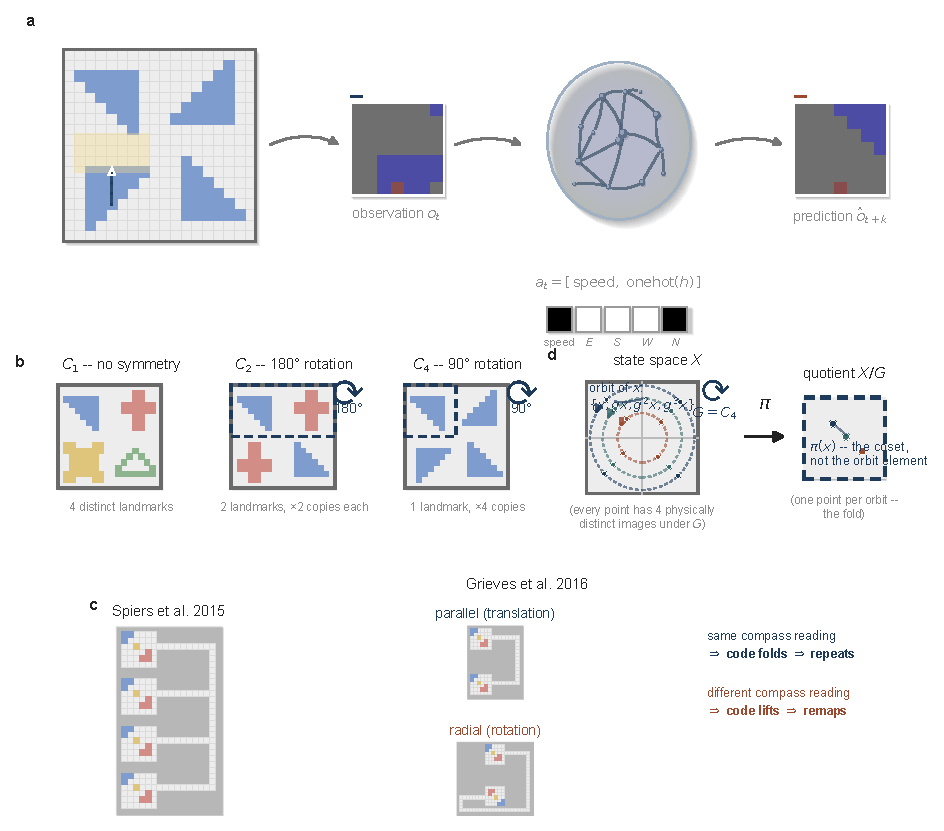
\includegraphics[width=\textwidth]{figures/fig1_overview.pdf}
\caption{\textbf{Overview.} (\textbf{a}) The pipeline: an agent moves through a symmetric arena
under actions drawn from a five-dimensional SpeedHD vector (Methods); a predictive RNN (pRNN)
receives the current $7\times7\times3$ egocentric observation $o_t$ and predicts the observation
$k$ steps ahead, $\hat{o}_{t+k}$. (\textbf{b}) The three arenas used throughout, named by their
landmark symmetry group: $C_1$ (four distinct landmarks, no symmetry), $C_2$ (one landmark pair
repeated under $180^\circ$ rotation), and $C_4$ (one landmark repeated four times under $90^\circ$
rotation); dashed outline marks a fundamental domain. (\textbf{c}) The animal phenomenon this study
explains: \citet{spiers2015} recorded a high degree of spatial repetition across four visually
identical compartments in a row; \citet{grieves2016} showed the same compartments arranged in
parallel produce repeated place fields, while arranging them radially, so that a rotation rather
than a translation relates them, produces remapping. (\textbf{d}) The central object of the
Theorem: a group $G$ (here $C_4$) partitions the state space $X$ into orbits; the quotient map
$\pi$ sends each orbit to a single point of $X/G$, discarding which physically distinct member of
the orbit the agent occupies.}
\label{fig:overview}
\end{figure}

\subsection{The phenomenon: identical rooms fold under translation and separate under rotation}

The cleanest place to see the idea is the geometry in which repeated place fields were first studied
in rodents. We built two closed $6\times6$ compartments joined by a corridor and gave them identical
interior landmarks, so the two rooms produced the same set of egocentric views: across all $144$
combinations of location and heading the observations coincided exactly. In one arrangement the rooms
are related by a translation, under which the compass reads the same in both; in the other by a
rotation, under which it does not. We trained networks on each arrangement, decoded which room the
agent occupied, and measured whether individual units repeated their firing fields between the rooms
(Fig.~\ref{fig:function}c).

The two arrangements gave opposite results ($n=8$ networks each). Under translation the fields
repeated almost exactly across the rooms (repetition $0.997$) and the room was very nearly
undecodable even by a nearest-neighbour classifier tested on cells it had already seen: $0.515$
against a chance of $0.5$. That residual is small, but it is real rather than noise ($p = 0.008$,
Wilcoxon, $n = 8$), and we neither round it away nor lean on it. It is the incomplete fold we
return to in the Discussion, where its size and cause are the subject. On any reading the two rooms
are very close to a single map. Under rotation the repetition vanished (repetition $-0.080$) and the
room decoded perfectly ($0.998$). Position within a room decoded well in both arrangements
($R^2 = 0.95$ and $0.79$), so neither network had stopped representing space. Every translation
network separated from every rotation network on all four measures (Mann--Whitney
$p = 1.6\times10^{-4}$, the exact two-sided floor at $n=8$ vs.\ $8$). \citet{grieves2016} reported
this same contrast in CA1, and here it follows from a single fact about how the compass transforms:
translation-invariant, rotation-equivariant (Methods; Limitations). The dissociation is visible
directly in the population geometry, with no decoder: an Isomap embedding of the wake population
state lands room B almost on top of room A under translation and pulls them an order of magnitude
apart under rotation (Supplementary Information, Fig.~S12).

The fold scales to the full four-compartment maze that \citet{spiers2015} recorded. We built four
identical closed rooms in a row, each a translation of the last, off a shared corridor, with every
view identical across the four rooms at matched local position and heading (verified exactly: zero
pixel mismatch over every room-interior cell and heading, Methods). A predictive network ($n=8$)
folded all four onto very nearly a single map (Fig.~\ref{fig:brain}a): against the $0.25$ chance of four alternatives, a
generalising decoder recovered the room at $0.262$ and a nearest-neighbour classifier tested on
cells it had already visited at $0.268$. As in the two-room maze, those residuals are small but not
nothing ($p = 0.008$ for both, Wilcoxon, $n = 8$), and we report them as such. Fields repeated across
the four rooms almost perfectly (repetition $0.994$) and within-room position stayed intact
($R^2 = 0.96$). Room identity is decoded only from room-interior states; the connecting corridor is
excluded for the reason given in Limitations. The two-room dissociation is thus not a small-$n$
artefact: at the rodent room count, translation-related identical rooms collapse completely, the
``high degree of spatial repetition'' that \citet{spiers2015} observed.

The account makes a further prediction, which we test in the model before asking whether it is
visible in real neurons. A city-block maze whose alleys run in two orthogonal orientations relates
same-orientation alleys by translation (the compass reads the same) and orthogonal alleys by a
$90^\circ$ rotation, so a repeating cell's fields should share a directional preference across
same-orientation alleys and not across orthogonal ones. A predictive network trained on this maze
confirms it: the directional index of same-orientation field pairs is positively correlated
($r = 0.62$; Fig.~\ref{fig:brain}b), and this is the model's own prediction, not a fit to animal
data. We then asked whether the signature is visible in real neurons, reanalysing the CA1 recordings
of \citet{hockeimer2023}. It is present, at a smaller magnitude ($r = 0.23$; $127$ pairs, $40$ cells,
$5$ rats), but the dataset cannot separate it from a conjunctive place-by-direction code that would
produce the same correlation without any folding; two controls make the ambiguity explicit
(Supplementary Information, Fig.~S10). We therefore report the CA1 correlation as \emph{consistent
with} the quotient but not diagnostic of it, and treat the model prediction, not the animal
reanalysis, as the load-bearing result of this section.

\begin{figure}[t]
\centering
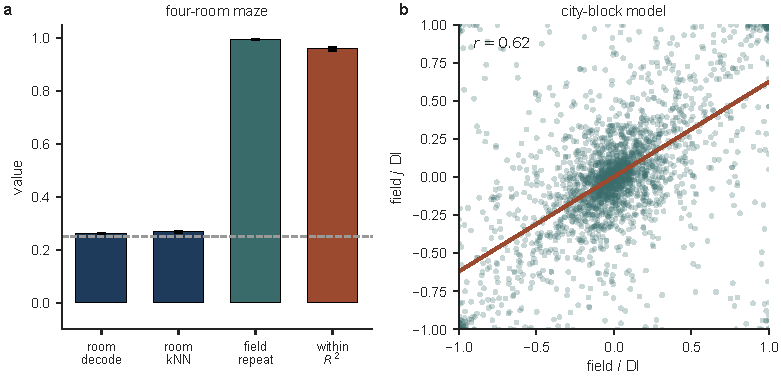
\includegraphics[width=\textwidth]{figures/fig6_brain.pdf}
\caption{\textbf{The predictive model reproduces place-field repetition.} (\textbf{a}) The
four-room maze of \citet{spiers2015}, model ($n=8$): four translation-related identical rooms fold
onto one map. The room decodes at $0.262$ by a generalising decoder and $0.268$ by a
nearest-neighbour classifier at cells it has already seen, against a chance of $0.25$ (dashed): a
small residual, but a reliable one ($p = 0.008$). Fields repeat across the rooms
(repetition $0.99$) and within-room position stays intact ($R^2=0.96$). (\textbf{b}) A predictive
network trained on a city-block maze shows the directional-repetition signature, predicted before
any comparison to animal data: the directional index of a field ($i$) against that of its
same-orientation partner ($j$) is positively correlated ($r=0.62$; scatter subsampled for display,
statistic from all pairs). Line, least-squares fit. An exploratory, non-diagnostic reanalysis of
real CA1 data testing the same prediction is in the Supplementary Information (Fig.~S10).}
\label{fig:brain}
\end{figure}

\subsection{Why a predictive map must fold: the quotient theorem}

The phenomenon has an explanation that needs no trained network at all. Return to the two identical
rooms. A trajectory through one room and the corresponding trajectory through its symmetry-related
copy generate, step for step, the same sequence of observations and the same sequence of encoded
actions. That is what ``identical rooms'' and ``an invariant compass'' mean together. A network is
a fixed function of that input sequence. If two histories feed it identical inputs, it must land in
identical internal states, and no reading of those states can afterwards recover which room the agent
was really in. The information was never in the stream. Everything below is this observation made
precise.

\noindent\textbf{Theorem} (folding onto the quotient)\textbf{.} \emph{Let a finite group $G$ act
freely on the arena's positions $X$, with a $G$-invariant start distribution, a $G$-equivariant
observation likelihood $p(o \mid x)$, and a policy measurable with respect to the agent's belief. If
the head-direction encoding is $G$-invariant, $\phi(h + g) = \phi(h)$ for every $g \in G$, then the
posterior over position given any history of observations and encoded actions is $G$-invariant, and
any decoder of the orbit element has accuracy at most $1/|G|$.}

\noindent\emph{Proof.} The action of $g \in G$ on trajectories, $\gamma \mapsto g\cdot\gamma$, is a
measure-preserving bijection: it fixes the invariant start distribution and the equivariant
transition and policy, and it leaves the sequence of observations and encoded actions unchanged,
because $G$-related positions are observationally identical and $\phi$ is $G$-invariant. Histories
ending at $x$ and at $g\cdot x$ therefore induce the same input sequence, so the network map, a
fixed function of that sequence, assigns them the same state, and the position posterior is constant
on each $G$-orbit. No function of the state separates orbit-mates, so an $|G|$-way phase decoder is
bounded by $1/|G|$.

The policy hypothesis is concrete, not abstract, and worth cashing out because it is easy to violate
by accident. Every trajectory in this paper is generated by a random walk with fixed action
probabilities (forward $0.60$, turn left $0.15$, turn right $0.15$, stop $0.10$; Methods), the same
at every position, heading, and copy of the fundamental domain. Such a policy is a function of
nothing the agent's belief could fail to represent, so it is trivially measurable with respect to
that belief. The hypothesis is not vacuous: it would fail for a policy that consulted information
outside the belief state, such as a script that explored one room more thoroughly than its $g\cdot$room
image, which would leak room identity into the action stream itself. Nothing in the experiments
does this; the walk cannot tell the rooms apart any better than the compass can.

The bound is an upper limit, not a prediction. It forbids exceeding the ceiling but does not force
the network to reach it, and the free-action assumption (no rotation fixes a cell, satisfied by the
even grid) is what gives every orbit exactly $|G|$ members. Two things the paper turns on are
therefore empirical, not entailed: that a \emph{predictive} objective drives the code to
\emph{saturate} the bound, where a reconstruction objective leaves it far below (a later section),
and that the folded code is folded rather than broken, since within-domain position survives. The
quotient is pinched between a proved ceiling and an empirical floor.

The proof turns on nothing but the sigma-algebra the (observation, action) stream generates, so the
ceiling is invariant to everything downstream of that stream, and this answers three worries at once.
It does not reference the observation's format: a $7\times7$ pixel patch, a higher-resolution render,
or a richer sensory channel are all $G$-equivariant whenever the arena is, so $G$-related histories
stay indistinguishable whatever the observation's dimensionality. It does not reference network
capacity: a larger or smaller decoder computes a function of the same aliased sequence, and no
capacity manufactures information the sequence does not carry, so a bigger network reaches the ceiling
faster, not past it. And it survives noise that leaves the equivariance intact. A compass corrupted
on $30\%$ of steps (a later section) changes how good each heading estimate is, not whether the
encoding stays invariant, and the fold does not move. What lifts the ceiling is only a channel that
breaks the equivariance itself: a statement about information content, not about richness, capacity,
architecture, or noise.

The theorem also tells us how to \emph{measure} the fold. Under folding onto $X/G$ the population
state satisfies $h(x) = h(R^2x)$, so no decoder can recover which element of the orbit $\{x, R^2x\}$
produced it. We therefore train a linear decoder for \emph{orbit phase}, holding out whole orbits
across cross-validation folds so the decoder must generalise a phase direction to positions it has
never seen. Chance is $0.500$; a fully folded code sits at the ceiling, an unfolded one well above it.
This is the readout the rest of the paper leans on, and the reason it can be trusted where single-cell
measures cannot is the subject of a later section.

\subsection{A design that separates equivariance from information}

The theorem hangs on one word, \emph{invariance}, and the experiment has to hold everything else
fixed to isolate it. Two hypotheses are on the table. If folding tracks how much the compass tells the
network, then any impoverished compass should fold. If it tracks equivariance, then only a compass
invariant under the arena's symmetry should fold, and one carrying the same information but not
invariant should not. These make opposite predictions, and the way to force them apart is a pair of
head-direction encodings matched in every respect but invariance.

That is what the four encodings do. Each network receives a $7\times7\times3$ egocentric view and a
five-dimensional SpeedHD action vector, $[\,\text{speed},\ \mathrm{onehot}(h)\,]$ with $h \in
\{\text{E},\text{S},\text{W},\text{N}\}$; we replace the heading block by $M\,\mathrm{onehot}(h)$ for
a fixed $4\times4$ matrix $M$, preserving dimensionality and column sums (Table~\ref{tab:encodings},
Fig.~\ref{fig:setup}a). \textit{full} keeps all four headings (two bits). \textit{const} discards
them (zero bits). The crucial pair is in between: \textit{axis} and \textit{parity} each collapse the
compass to a single bit, with identical entropy and identical activation statistics. They differ only
in \emph{which} headings they group together, and so in whether the bit is invariant under the
$180^\circ$ rotation $R^2$. \textit{axis} groups $\{E,W\}$ against $\{N,S\}$ and is invariant under
$R^2$; \textit{parity} groups $\{E,S\}$ against $\{W,N\}$ and is not. If information drives the fold,
they behave alike. If invariance drives it, \textit{axis} folds and \textit{parity} does not. Nothing
else about the two differs.

\begin{table}[t]
\centering
\caption{The four head-direction encodings. \textit{axis} and \textit{parity} are matched at
one bit and differ only in invariance.}
\label{tab:encodings}
\begin{tabular}{lccc}
\toprule
encoding & bits & $C_2$-invariant & $C_4$-invariant \\
\midrule
\textit{full} (E,S,W,N)            & 2.0 & no  & no  \\
\textit{parity} (\{E,S\} vs \{W,N\}) & 1.0 & no  & no  \\
\textit{axis} (\{E,W\} vs \{N,S\})   & 1.0 & \textbf{yes} & no \\
\textit{const}                     & 0.0 & yes & \textbf{yes} \\
\bottomrule
\end{tabular}
\end{table}

\begin{figure}[t]
\centering

\includegraphics[width=\textwidth]{figures/fig1_setup.pdf}
\caption{\textbf{Design and phenotype.} (\textbf{a}) The four head-direction encodings, as
$4\times4$ transforms of the one-hot heading block $\{$E,S,W,N$\}$; grey level is the matrix
weight. \textit{full} is the identity (two bits); \textit{parity} and \textit{axis} collapse the
compass to one bit with different partitions; \textit{const} discards it. \textit{axis} and
\textit{const} are invariant under the $180^\circ$ rotation and fold the $C_2$ arena;
\textit{const} is the only encoding invariant under the full $C_4$ group. \textit{axis} and
\textit{parity} carry identical entropy (one bit) and differ only in invariance. (\textbf{b}) Mean
firing-rate maps (smoothed, peak-normalised) of example units. Fields are single and sharp when
the code does not fold, and repeat at the symmetry-related locations, once under $C_2$
(\textit{axis} encoding) and four times under $C_4$ (\textit{const}). Units are representative;
the complete unselected set for each condition is given in the Supplementary Information.}
\label{fig:setup}
\end{figure}

\subsection{Predictive learning grows place cells, and symmetry makes them repeat}

Trained on prediction alone, the networks develop units with localised spatial firing fields, the
place cells reported for this objective by \citet{levenstein2024} (Fig.~\ref{fig:setup}b). In the
asymmetric arena under the full compass, about $480$ of the $500$ units carry a place field (a median
of about two fields per unit). The effect of symmetry is already visible in the rate maps, before any
decoder is applied. When the arena is symmetric and the head-direction encoding is invariant to that
symmetry, the fields repeat: a unit in the $C_2$ arena under \textit{axis} fires at a location and
again at its $180^\circ$ image, and a unit in the $C_4$ arena under \textit{const} fires at all four
$90^\circ$ copies. A single unit reports every member of a symmetry orbit as the same place. The
sections that follow quantify this and isolate what controls it.

\subsection{Matched bits, opposite maps: equivariance is the cause}

With the readout in hand and the encodings matched, the whole experiment fits in one table. Orbit-phase
decoding separates the encodings exactly as invariance, not information, predicts
(Table~\ref{tab:phase}, Fig.~\ref{fig:dissoc}). \textit{full} and \textit{parity} stay high in every
arena. The invariant encodings, \textit{axis} and \textit{const}, fall to chance in precisely the
arenas whose symmetry they cannot break.

\begin{table}[t]
\centering
\caption{Orbit-phase decoding accuracy (chance $=0.500$). $n=10$ per cell for s1 and s2,
$n=8$ for s4.}
\label{tab:phase}
\begin{tabular}{lcccc}
\toprule
arena & \textit{full} & \textit{parity} & \textit{axis} & \textit{const} \\
\midrule
s1 ($C_1$, no symmetry) & 0.981 & 0.972 & 0.971 & 0.966 \\
s2 ($C_2$)              & 0.978 & 0.955 & \textbf{0.552} & \textbf{0.552} \\
s4 ($C_4$)              & 0.984 & 0.933 & \textbf{0.544} & \textbf{0.521} \\
\bottomrule
\end{tabular}
\end{table}

\begin{figure}[t]
\centering
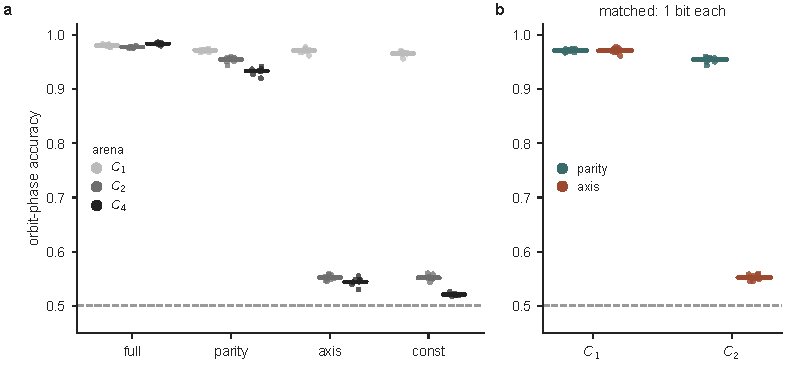
\includegraphics[width=\textwidth]{figures/fig2_dissociation.pdf}
\caption{\textbf{Invariance, not information, folds the code.} (\textbf{a}) Orbit-phase decoding
accuracy for every trained network (one dot per network; horizontal bar, group mean), by
head-direction encoding and arena; chance $0.5$ (dashed). \textit{full} and \textit{parity} stay
high in every arena, whereas the invariant encodings \textit{axis} and \textit{const} fall to
chance in the symmetric arenas. (\textbf{b}) The matched-entropy contrast: \textit{axis} and
\textit{parity} carry one bit each and are indistinguishable in the $C_1$ arena (both
$\approx0.97$) but separate completely in $C_2$ (\textit{parity} $0.955$, \textit{axis} $0.552$;
every \textit{parity} network scores above every \textit{axis} network, Mann--Whitney
$p = 1.1\times10^{-5}$). Data of Table~\ref{tab:phase}.}
\label{fig:dissoc}
\end{figure}

The decisive comparison is the matched pair. In the $C_2$ arena, \textit{axis} and \textit{parity}
carry the same entropy (one bit) and the same information about the current heading, yet they differ
by $0.403$ in phase accuracy ($0.552$ against $0.955$). What separates them is equivariance:
\textit{parity}'s bit is informative about orbit phase, since it distinguishes a position from its
$180^\circ$ image, whereas \textit{axis}'s bit is invariant under that rotation and so carries none.
The separation is complete: every \textit{parity} network scores above every \textit{axis} network
(Mann--Whitney $U=0$, $p = 1.1\times10^{-5}$, the exact two-sided floor at $n=10$ vs.\ $10$;
$p = 3.2\times10^{-5}$ after Bonferroni correction across the three arenas). And in the $C_1$ arena,
where there is no symmetry to collapse onto, the same two encodings are indistinguishable
($\Delta = 0.000$, $p = 0.97$). That $C_1$ null is what licenses the causal reading: \textit{axis}
does not degrade spatial coding in general; it degrades it exactly when the arena has a symmetry under
which \textit{axis} is invariant. The chance-level reading is not an artefact of the linear decoder. A
$k$-nearest-neighbour decoder and a multi-layer perceptron also sit at chance for the invariant
encodings, and recover phase for the non-invariant ones (Supplementary Information). The orbit-phase
information is absent from the folded code, not merely hidden from a linear readout.

\subsection{The $C_4$ map hits the group-theoretic $1/|G|$ ceiling}

The theorem makes a sharper prediction than ``the code folds.'' A code folded onto $X/G$ can name the
coset but not the element within it, so a $|G|$-way phase decoder is bounded by exactly $1/|G|$, a
number with no free parameters. The $C_4$ arena, read through its own four-way quotient (chance
$0.250$), is where this is testable, and the networks land on it (Table~\ref{tab:c4},
Fig.~\ref{fig:ceiling}). \textit{const}, the only $C_4$-invariant encoding, falls to the $C_4$ floor
($0.275$, just above $0.250$). \textit{axis}, invariant under $C_2$ but not $C_4$, falls only to the
$C_2$ ceiling of $0.5$ ($0.482$). The non-invariant encodings stay high. The folded values sit a few
percent above their predicted floors rather than exactly on them, and that residual is real signal
rather than decoder bias: across networks, $C_2$ phase accuracy under \textit{axis} is $0.552$ against
its floor of $0.500$ (one-sample $t$-test, $t(9) = 34.8$, $p = 6.6\times10^{-11}$, $n = 10$), and
under \textit{const} $0.552$ ($t(9) = 35.2$, $p = 6.0\times10^{-11}$). The fold is very close to, but
not exactly, complete. The decisive quantity for the account is which floor each encoding falls to,
not the residual's exact size (Discussion).

\begin{table}[t]
\centering
\caption{$C_4$ four-way phase decoding in the s4 arena (chance $= 0.250$); $n = 4$ networks per encoding.}
\label{tab:c4}
\begin{tabular}{lccc}
\toprule
encoding & invariance & measured & predicted ceiling \\
\midrule
\textit{full}   & none          & 0.918 & --- \\
\textit{parity} & none          & 0.860 & --- \\
\textit{axis}   & $C_2$ only    & \textbf{0.482} & 0.500 \\
\textit{const}  & $C_2$ and $C_4$ & \textbf{0.275} & 0.250 \\
\bottomrule
\end{tabular}
\end{table}

\begin{figure}[t]
\centering
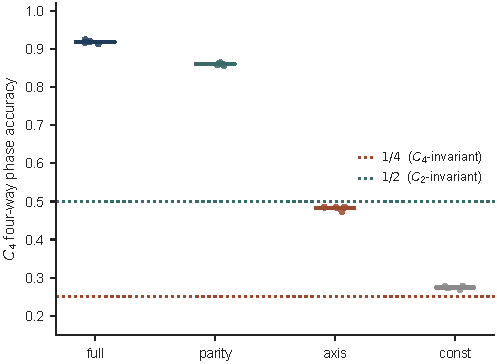
\includegraphics[width=0.62\textwidth]{figures/fig_ceiling.pdf}
\caption{\textbf{The $C_4$ arena reproduces the group-theoretic ceiling.} Four-way orbit-phase
accuracy in the $C_4$ arena (one dot per network; bar, mean; chance $0.25$). A code folded onto
$X/G$ can name the coset but not the orbit element, so a $|G|$-way decoder is bounded by $1/|G|$.
\textit{const}, invariant under the full $C_4$ group, falls to the $1/4$ ceiling (dotted); the
$C_2$-invariant \textit{axis} falls to the $1/2$ ceiling; \textit{full} and \textit{parity}, not
invariant, stay high. Ceilings are the group-theoretic predictions, not fits. $n = 4$ networks per encoding.}
\label{fig:ceiling}
\end{figure}

This also resolves what \textit{const} in the $C_4$ arena looked like under the wrong readout. Read
through the $C_2$ quotient it appeared dead; read through the $C_4$ quotient it is plainly a live
spatial code, its $C_4$ fundamental-domain $R^2$ is $+0.646$ (minimum $+0.535$ across the four
\textit{const} networks), and its four-way phase accuracy of $0.275$ sits at the $C_4$ chance floor.
What looked like a dead code was a code folded onto a larger quotient than the readout was built to
see. We flag this because a $G$-folded code and a code that has stopped representing space are easy to
confuse, and only the second is a failure.

\subsection{A folded map, not a broken one}

Everything so far is a negative: a decoder that cannot recover orbit phase. A negative is a weak thing
to build on, because a merely degraded code also fails a decoder. So we asked the positive question. If
the quotient law is right, a folded code is not a poor map of the arena; it is a \emph{faithful map of
a different space}. That is a claim about geometry, and it can be tested directly.

The folded networks have not stopped representing space. For $104$ of the $112$ networks,
$\max(R^2_{\text{raw}}, R^2_{\text{domain}}) \ge 0.81$: the folded codes still linearly encode position
\emph{within the fundamental domain}, and have merely discarded which copy of it the agent occupies
(Fig.~\ref{fig:manifold}). The eight exceptions are \textit{const} in the $C_4$ arena, which fails both
$C_2$-based readouts ($R^2_{\text{raw}} = -0.069$, $R^2_{\text{domain}} = -0.589$) not because it has
stopped coding space but because it is folded by the full $C_4$ group, which a $C_2$ decoder cannot see.
Domain position and orbit phase move independently across every network and encoding (Supplementary
Information, Fig.~S11), which is the coset-versus-phase signature of a fold rather than a dead code.

\begin{figure}[t]
\centering
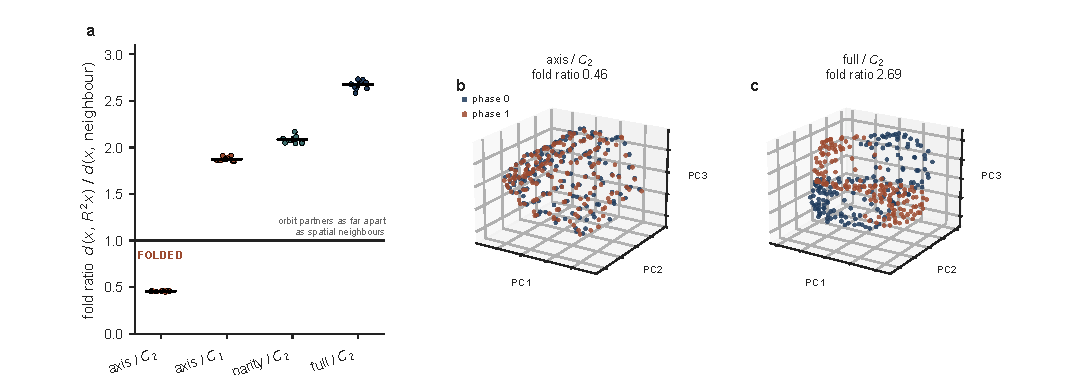
\includegraphics[width=\textwidth]{figures/fig_manifold.pdf}
\caption{\textbf{The fold, seen geometrically.} (\textbf{a}) The fold ratio: the distance between
a cell's population state and that of its $180^\circ$ image, in units of the distance to an
adjacent cell. One dot per network, $n=10$ per condition; bar, mean; whiskers, $95\%$ bootstrap
interval. Below one, orbit partners sit closer together than spatial neighbours do, which is what
folding means. Only \textit{axis} in the $C_2$ arena is below one ($0.457 \pm 0.004$); the same
encoding with no symmetry to fold onto is not (\textit{axis}/$C_1$, $1.872$), nor is
\textit{parity}/$C_2$ ($2.083$), nor \textit{full}/$C_2$ ($2.675$). The ratio is computed in the
full hidden space, so it is not an artefact of the projection used to plot it: the folded case
reads below one and every non-folded case above one under nonlinear embeddings
(Isomap, t-SNE) as well as PCA. (\textbf{b}, \textbf{c}) Position-conditioned population manifold
of the most- and the least-folded condition (one point per arena cell, PCA to three dimensions,
coloured by $C_2$ orbit phase), illustrative; the fold ratio in (a) is the quantitative claim. The
two phases superimpose under \textit{axis}/$C_2$ and occupy separate regions under
\textit{full}/$C_2$. We reduce with PCA because the claim is metric, that two positions coincide,
and unlike neighbour-graph embeddings PCA preserves distances rather than reshaping them.}
\label{fig:manifold}
\end{figure}

To test the positive claim we took, for each network, the population state averaged at every arena cell
and measured the geodesic distances between those states. We then asked which of two candidate metrics
those neural distances reproduce: the arena's own metric $d_X$, or the quotient metric
$d_{X/G}(x,y) = \min_{g \in G} \lVert x - g\!\cdot\!y \rVert$. Fit is Kruskal stress at an optimal scale,
since neural units are arbitrary and an isometry is only ever defined up to a scale factor (Methods).

The head-direction encoding decides which space the manifold is a map of, and it does so with one
systematic exception we report rather than round away. Taking for each network whichever of $d_X$,
$d_{X/C_2}$ and $d_{X/C_4}$ fits its geometry best, $103$ of $112$ networks are assigned by their
encoding alone: \textit{full} and \textit{parity} map $X$; \textit{axis} maps $X/C_2$; \textit{const}
maps $X/C_4$. The nine that are not are almost all one cell: every \textit{axis} network in the $C_4$
arena ($8/8$) is fitted better by $X/C_4$ than by the $X/C_2$ its encoding predicts. This disagrees
with our decoder, which puts the same networks at $0.482$, the $C_2$ ceiling. The decoder is the
measure we trust here, because $d_{X/G} \le d_X$ pointwise, so a \emph{larger} group can always fit a
compressed code better, biasing the stress comparison toward over-folding in exactly this nested case.
We flag the disagreement, we do not resolve it here, and no claim in this paper rests on the geometry
metric where it and the decoder part company.

Where they agree, the geometry is unambiguous. In the $C_2$ arena the folded \textit{axis} code fits
the quotient at stress $0.190$ against $0.468$ for the arena, the mirror image of \textit{full}, which
fits the arena at $0.097$ against $0.485$ for the quotient (Fig.~\ref{fig:isometry}a). The compass does
not degrade the map; it selects the space the map is of. One artefact had to be excluded first. Because
$d_{X/G} \le d_X$ pointwise, any group shrinks long distances, so a code whose neural distances merely
saturate at long range would prefer a quotient metric for reasons unrelated to symmetry. We therefore
built a sham group of the same order: a translation by half the arena, which compresses distances
exactly as $C_2$ does but is a symmetry of no arena here. The folded code prefers the true symmetry
over the sham by $0.343$ (Fig.~\ref{fig:isometry}b), while the unfolded codes prefer neither. The
preference is for the group, not for the compression. The same claim survives with no metric at all:
the cosine between the population state at $x$ and at its $180^\circ$ image is $0.990$ under
\textit{axis} and $0.741$ under \textit{parity} in the $C_2$ arena (Mann--Whitney $U = 100$,
$p = 1.1\times10^{-5}$; Fig.~\ref{fig:isometry}c). Under the invariant encoding the orbit has collapsed
to a point; under the encoding carrying the same one bit it has not. The same collapse appears as a
glued fundamental domain in a nonlinear Isomap embedding: a position and its $180^\circ$ image sit
at $0.17$--$0.18$ of a random pair's distance under \textit{axis}, against $0.85$--$0.89$ under
\textit{full} (Supplementary Information, Fig.~S8). It is a property of the geometry, not of the
projection used to see it.

\begin{figure}[t]
\centering

\includegraphics[width=\textwidth]{figures/fig_isometry.pdf}
\caption{\textbf{The folded manifold is a map of the quotient.} One dot per network ($n=10$ per
condition, $8$ for $C_4$); stress is Kruskal stress-1 at optimal scale, lower is a better fit.
(\textbf{a}) Fit to the arena metric $d_X$ against fit to the quotient metric $d_{X/C_2}$, with the
line of equal fit. \textit{full} and \textit{parity} lie above it, so they are better described as
maps of $X$; \textit{axis} lies below it, so it is better described as a map of $X/C_2$. Dotted
line, the stress returned when the code's spatial content is destroyed by shuffling, a reachable
ceiling. (\textbf{b}) The control for the compression artefact: $d_{X/G} \le d_X$ pointwise, so any
group shrinks long distances. A sham order-2 group (translation by half the arena) compresses
identically but is not a symmetry, and the folded code prefers the true $C_2$ over it by $0.343$.
(\textbf{c}) The same claim without any metric: the cosine between the population state at $x$ and
at its $180^\circ$ image. Under \textit{axis} in the $C_2$ arena it is $0.990$, so the orbit is one
point; under \textit{parity}, which carries the same one bit, it is $0.741$.}
\label{fig:isometry}
\end{figure}

The geometry also separates the theorem's two conditions, which the decoder cannot. \textit{axis} folds
the \emph{geometry} by $C_2$ even in the $C_1$ arena, where there is no symmetry at all (it prefers
$d_{X/C_2}$ over the sham by $0.145$, and its orbit cosine is $0.811$), and yet orbit phase there stays
decodable at $0.971$. An invariant compass pulls symmetry-related states together wherever it is used;
it is the \emph{observations} being equivariant that also destroys the information. Only where both
hold does the code fold completely, which is the intersection $G$ the introduction promised, now seen
in the geometry.

\subsection{Prediction builds the fold; reconstruction does not}

The fold, so far, is a property of the inputs. Whether a network actually builds it turns out to depend
on what the network is trained to do, and this is the one manipulation that could have shown the fold is
an accident of the architecture rather than a consequence of prediction.

Start with the inputs alone. Call two states $(x,h)$ and $(x',h')$ \emph{input-equivalent} if they
produce the same $7\times7$ observation and the same HD encoding. A code is a function of its inputs, so
no decoder can separate input-equivalent states, and phase decoding is bounded above by

\begin{equation}
\mathrm{acc}_{\max} \;=\; \tfrac12 + \tfrac12 \, \Pr_{(x,h)}\!\big[\,(x,h) \not\sim (R^2x,\, h+2)\,\big],
\label{eq:bound}
\end{equation}

the fraction of orbit pairs the input distinguishes. Evaluating the right-hand side on the arenas
themselves, by enumerating all $324\times4$ states and hashing their observations, takes no training
at all, and it predicts the trained networks to a mean absolute error of $0.031$ across the twelve cells
(Table~\ref{tab:bound}). It also settles a number that would otherwise look like a failure: in the $C_1$
arena \textit{axis} reaches $0.971$ rather than $1.000$ because $6.6\%$ of states there are
\emph{accidentally} observationally identical to their $C_2$ partner, putting the bound at $0.967$.
\textit{axis} and \textit{const} sit exactly on it. They were not failing to fold; they were folding on
precisely the ambiguous fraction.

\begin{table}[t]
\centering
\caption{The bound of Eq.~\ref{eq:bound}, computed from the arenas with no free parameters,
against the trained networks. Every encoding falls to the accuracy its input-distinguishability
predicts; the mean absolute error across the twelve cells is $0.031$. (We report the bound as a
bound, not a fit: the predicted values are near-degenerate, clustered at $1.0$ and at the
folding floors, so a correlation coefficient across cells would merely register that
separation.)}
\label{tab:bound}
\begin{tabular}{llccc}
\toprule
arena & encoding & distinguishable & predicted & measured \\
\midrule
s1 & \textit{full} / \textit{parity} & 1.000 & 1.000 & 0.981 / 0.972 \\
s1 & \textit{axis} / \textit{const}  & 0.934 & 0.967 & 0.971 / 0.966 \\
s2 & \textit{full} / \textit{parity} & 1.000 & 1.000 & 0.978 / 0.955 \\
s2 & \textit{axis} / \textit{const}  & 0.000 & 0.500 & 0.552 / 0.552 \\
s4 & \textit{full} / \textit{parity} & 1.000 & 1.000 & 0.984 / 0.933 \\
s4 & \textit{axis} / \textit{const}  & 0.000 & 0.500 & 0.544 / 0.521 \\
\bottomrule
\end{tabular}
\end{table}

The bound is an upper limit, and a network is free to discard information its loss does not reward. To
see whether the objective is what recruits the compass, we held the wiring, the compass, and the
training data fixed and changed only the rollout horizon $k$. At $k=0$ the target is the network's own
current observation: a pure autoencoder, with the same architecture and the same compass. At $k\ge1$ it
must predict a future observation. The result is a switch (Table~\ref{tab:horizon}, Fig.~\ref{fig:function}a). At
$k=0$ the input still separates $1228$ of the $1296$ states under \textit{full}, so the compass is right
there, yet all four encodings collapse to within $0.005$ of one another, landing on the
\emph{observation-only} bound of $0.500$; the spread across encodings is $0.0052$ at $k=0$ against
$0.427$ at $k=5$. The compass is not absent under reconstruction; it is \emph{discarded}: reconstructing
$o_t$ never requires knowing which of two identical places you occupy, whereas predicting $o_{t+1}$ does,
and one step is enough. Everything downstream, the ceiling, the replay, and the lesion effects, is
therefore not a property of a network that happens to also predict. It is what a fixed architecture
does \emph{because} the objective is prediction.

\begin{table}[t]
\centering
\caption{Orbit-phase decoding in the $C_2$ arena as a function of prediction horizon $k$
(chance $= 0.500$, $n = 6$ per cell).}
\label{tab:horizon}
\begin{tabular}{lccccc}
\toprule
$k$ & \textit{full} & \textit{parity} & \textit{axis} & \textit{const} & \textit{axis} vs \textit{parity} \\
\midrule
0 (autoencoder) & 0.536 & 0.541 & 0.539 & 0.539 & $p = 0.59$ \\
1 & 0.975 & 0.941 & 0.545 & 0.546 & $p = 0.00216$ \\
3 & 0.968 & 0.947 & 0.548 & 0.545 & $p = 0.00216$ \\
5 & 0.978 & 0.953 & 0.553 & 0.551 & $p = 0.00216$ \\
\bottomrule
\end{tabular}
\end{table}

The same switch appears in place-field size, and it matters for a common reading of the predictive
horizon. If $k$ behaved like a successor-representation discount, place fields should widen smoothly
with it, giving the kind of representation-scale gradient reported along the hippocampal dorsoventral
axis \citep{kjelstrup2008}. Instead mean field area (\textit{full}, $C_2$) jumps once and stops:
$33.8 \pm 1.6$ cells at $k=0$, $40.7 \pm 1.0$ at $k=1$, and no further ($42.1 \pm 1.0$ at $k=3$,
$39.7 \pm 0.7$ at $k=5$; \texttt{field\_area\_horizon.csv}). Prediction versus no prediction sets field
size once, the same way it sets the fold; how far ahead the network predicts does not additionally
scale it, at least across this range of $k$ and at fixed hidden size. This architecture does not offer
the discount-gradient account of the dorsoventral axis for free.

\begin{figure}[t]
\centering

\includegraphics[width=\textwidth]{figures/fig3_function.pdf}
\caption{\textbf{Functional consequences of the fold.} (\textbf{a}) Orbit-phase decoding
accuracy vs prediction horizon $k$ in the $C_2$ arena (chance $0.5$); the non-invariant
encodings (\textit{full}, \textit{parity}) resolve the fold at $k \geq 1$, the invariant ones
(\textit{axis}, \textit{const}) stay near chance. (\textbf{b}) Coverage of the self-generated
offline trajectory as a fraction of a wake path of equal length (dashed line, wake). Both step
up at $k = 1$ and are ordered by how much of the compass the encoding keeps; points are mean
$\pm$ s.e.m., $n = 6$. (\textbf{c}) Place-field repetition across two observationally identical
compartments ($n = 8$ each): under translation the fields repeat and the room barely decodes
($0.515$ against a chance of $0.5$; the residual is small but reliable), under rotation the fields do
not repeat and the room decodes perfectly; within-room
position ($R^2$) stays high in both. Dots are individual networks.}
\label{fig:function}
\end{figure}

\subsection{Map and replay are the same variable, read two ways}

A predictive network can be run offline, driven by its own predicted observation, to generate
trajectories without moving through the arena \citep{levenstein2024}. Its offline behaviour tracks the
fold. Both the coverage of the arena (relative to a waking path of equal length) and the sequenceness
of the rollout (the rank correlation between principal-axis position and time, against time-shift and
cell-shuffle nulls) step up between $k=0$ and $k=1$, the same range as orbit-phase accuracy, and
both fall as the compass is weakened (Fig.~\ref{fig:function}b). Coverage at $k=1$ runs $1.30$, $0.80$,
$0.45$ and $0.31$ times waking under \textit{full}, \textit{parity}, \textit{axis} and \textit{const},
the order in which the code folds, and sequenceness falls from $0.53$ under \textit{full} (waking
$0.56$; its own cell-shuffle floor $0.26$) to $0.21$ under \textit{axis} (floor $0.17$), approaching
that floor without reaching it.

One caveat belongs beside the coverage numbers, not in a supplement. A shuffled rollout covers
$1.57\times$ the waking path, more than \emph{any} of our networks, the best of which reaches
$1.30\times$. Coverage rewards incoherence: a trajectory that teleports visits more of the arena than
one that walks. It is a measure of extent, not of structure, and cannot on its own evidence structured
replay. Sequenceness is the readout that carries that claim, and it is the one with a null the real
networks clear (\textit{full} $0.53$ against a floor of $0.26$). We report coverage because the
$k=0 \to k=1$ step is real and matters, and we report its null because it is unflattering.

This is more than a shared horizon; it is the same variable measured twice. The $k$-sweep that takes
the map from the observation-only bound to a resolved map (Table~\ref{tab:horizon}) is the identical
manipulation that takes offline coverage from $0.37\times$ waking under the autoencoder to full
engagement under one step of prediction, and the \textit{full}/\textit{parity}/\textit{axis}/%
\textit{const} order in which encodings fold the map is the order in which they lose the replay. A
predictive objective does not separately grow a spatial map and a capacity to generate offline
activity. It grows one thing, self-motion integration, recruited because prediction requires it, and
the map and the replay are two readouts of it. Reconstruction, the only objective tested here that
removes the mechanism, removes both readouts at once and by the same amount. This is the sense in which
predictive learning is a unifying account of the spatial code rather than a fact about place-field
statistics: not that it produces a map and, separately, produces replay, but that the one thing it
does is read out as both.

Two limits on the replay claim. Sequenceness is scored as $|\mathrm{Spearman}(x(t), t)|$, an absolute
value, so it measures whether a rollout is an ordered sweep at all and is blind by construction to
whether that sweep runs forward or in reverse. We therefore make no claim here about forward versus
reverse replay; real reverse replay is reward-triggered \citep{fosterwilson2006, dibabuzsaki2007} and
this network has no reward signal, so the account predicts its sweeps should not show that
reward-linked form, but testing it needs a directional statistic we have not built.

\subsection{The fold survives a noisy compass and arises from a learned one}

The head-direction signal so far is a noiseless oracle, whereas a biological compass drifts and is
re-anchored by vision. Two tests ask whether the fold depends on that idealisation, and it does not.

First, noise. We retrained the $C_2$ networks with the reported heading corrupted on $30\%$ of steps
(rotated by a random $\pm 90^\circ$ before encoding). The dissociation is preserved: orbit-phase
decoding is $0.556$ under \textit{axis} and $0.922$ under \textit{parity}, a separation of $0.367$
that remains complete (Mann--Whitney $U = 0$, $p = 0.0022$ at $n = 6$ vs.\ $6$). Relative to the clean
networks the separation narrows only slightly (from $0.403$), driven by a small drop in \textit{parity}
resolution ($0.955 \to 0.922$) while the folded \textit{axis} code is unchanged ($0.552 \to 0.556$;
Fig.~\ref{fig:generality}a). A compass corrupted on a third of steps folds the same symmetries a clean
one does.

Second, and more strongly, we removed the oracle entirely. Rather than degrade a supplied compass, we
withheld absolute heading and gave the network only \emph{angular velocity}, the per-step turn, so
it had to integrate its own heading, unanchored, as a path-integrating head-direction system does. An
integrated compass is defined only up to a global rotation, so it is invariant under any rotation of the
arena by construction and cannot, by itself, separate a position from its symmetry image. The learned
compass reproduces the fold from first principles. In the asymmetric arena it decodes orbit phase almost
perfectly ($0.971$, $n=10$), because the arena's unique landmarks anchor absolute position. In the $C_2$
arena it falls to chance ($0.526$, $n=10$): raw position is not recoverable ($R^2 = -0.08$) while
position \emph{within} the fundamental domain is ($R^2 = 0.89$), so the network knows where it is inside
a copy, not which copy. In the $C_4$ arena it folds likewise ($0.523$, $n=8$; $R^2_{\text{domain}} =
-0.47$, the fourfold signature a $C_2$ decoder cannot see; Fig.~\ref{fig:generality}b). The fold is
therefore not an artefact of imposing an invariant encoding: it is the generic consequence of a
self-motion signal that carries no absolute reference under the arena's symmetry, the situation of a
biological compass that has lost its landmark anchor. The hand-designed encodings are a controlled way
to dial that invariance; the learned compass shows the invariance is where a real self-motion signal
already lives.

\begin{figure}[t]
\centering
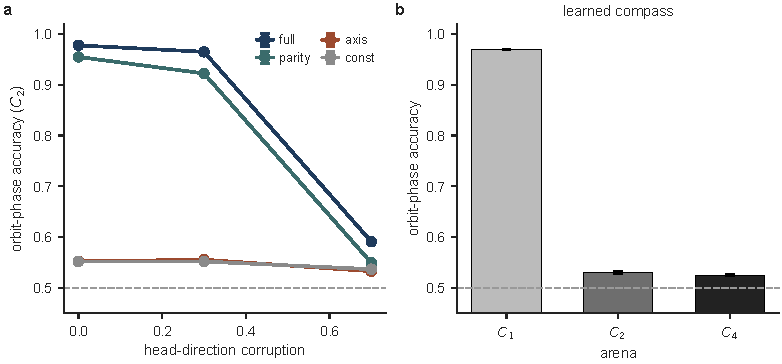
\includegraphics[width=0.86\textwidth]{figures/fig5_generality.pdf}
\caption{\textbf{The quotient survives a degraded and a learned compass.} (\textbf{a}) Compass
corruption \emph{during training}: orbit-phase accuracy in the $C_2$ arena for networks that
\emph{developed} with a heading signal randomised on a given fraction of steps (chance $0.5$,
dashed). The non-invariant encodings (\textit{full},
\textit{parity}) degrade smoothly, while the invariant ones (\textit{axis}, \textit{const}) stay
pinned at chance. This is a network that grew up with an unreliable compass, and it is \emph{not}
the lesion: an adult lesion is modelled by \emph{silencing} the compass at test time
(Fig.~\ref{fig:lesion}), because randomising a compass an adult network already trusts contradicts
its egocentric view rather than falling silent, and drives it off its training manifold.
(\textbf{b}) A learned, angular-velocity compass, by arena: it resolves $C_1$
($0.97$) but folds $C_2$ and $C_4$ to chance, building the quotient with no imposed encoding.}
\label{fig:generality}
\end{figure}

\subsection{Two causes leave two fingerprints, and no cell type carries the fold}

The claim that folding is driven by equivariance and not information has, so far, rested on one readout.
It can be made with a second that moves the \emph{other} way, which is a stronger argument than either
alone. Decompose each unit's variance into what a purely \emph{additive} model of place and heading
explains and what the full \emph{conjunctive} model explains; the difference is nonlinear mixed
selectivity, the part of the code that is a joint function of place and heading and of neither
separately. It behaves nothing like the fold. Mixed selectivity is ordered by how much the compass
\emph{knows}: it rises as the compass is impoverished ($0.235$ under \textit{full} at two bits,
$0.292$ under \textit{parity}, $0.331$ under \textit{axis} at one bit each, $0.333$ under \textit{const}
at none), and the fraction of units carrying it goes from $91\%$ to $97\%$, while position-only variance
falls in step ($0.505 \to 0.312$). Heading that the compass does not supply must be recovered from
the conjunction of where the agent is and what it sees, and a code forced to do that mixes its variables.
The rise is almost indifferent to symmetry: $+0.085$ in the $C_1$ arena against $+0.096$ in
$C_2$, so $88\%$ of it is present where nothing can fold.

Set the two readouts side by side and they come apart completely. Under \textit{axis} and
\textit{parity}, the same one bit, phase decoding reads $0.552$ and $0.955$ (a difference of
$0.40$), while mixed selectivity reads $0.331$ and $0.292$ (a difference of $0.04$). Across the three
arenas at fixed encoding, phase decoding moves from $0.971$ to $0.552$ while mixed selectivity barely
stirs ($0.310$, $0.331$, $0.325$). \emph{Phase decoding is blind to information and tracks equivariance;
mixed selectivity is blind to equivariance and tracks information.} They are two fingerprints of two
causes, in the same networks. The consequence for reading real data is worth stating plainly, because it
is otherwise got backwards: a folded code \emph{is} more mixed than an unfolded one, but not because it
folded. The two travel together only because a compass that fails to break a symmetry usually also
carries less information, and it is the missing information, not the surviving symmetry, that forces the
mixing.

The same lesson, that an invariant compass makes the code look symmetric whether or not the arena is,
disqualifies three further single-cell readouts we tried (rotational autocorrelation, isotypic odd
power, and spatial representational similarity): each reports a fold in the $C_1$ arena, where none can
exist. We relegate them and the reasoning to the Supplementary Information, and report orbit-phase
decoding, whose null does survive the $C_1$ arena, as the primary readout throughout.

Finally, if repetition were simply a cell type seen twice, the fold should live in a subpopulation. It
does not (Fig.~\ref{fig:fold}). Scored unit by unit as the correlation of a rate map with its own
$180^\circ$ rotation, across all $56{,}000$ units the fold is everywhere: in the $C_2$ arena under
\textit{axis}, $93.1\%$ of units score above $0.8$ (median $0.94$, fifth percentile $0.77$), while under
\textit{full}, the reachable null, $54.3\%$ of units fall \emph{below} $0.2$ (median $0.09$), so the
readout is free to return the negative answer. And the fold does not track cell type: the most
boundary-tuned quartile of units folds at $0.947$ and the least at $0.923$, a difference of $0.024$ on an
effect of size $0.9$, and the correlation between border tuning and folding is $r = 0.16$ (under $3\%$ of
the variance), no larger than its correlations with spatial information ($0.25$) or nonlinear mixing
($-0.15$). No cell class carries the fold, because it is a property of what the code can distinguish, not
of any unit's receptive field.

Cast in the standard hippocampal metrics, the same population reads as a realistic map that fails to
remap exactly where the compass is blind. The population-vector correlation \citep{leutgeb2005} between a
position and its symmetry image is $0.98$ under the invariant encodings in the $C_2$ and $C_4$ arenas
and about $0.28$ under \textit{full}, with \textit{parity} intermediate ($0.58$ in $C_2$;
Supplementary Information, Fig.~S13). Fields per
unit rise from $1.78$ under \textit{full} in $C_1$ to $3.39$ under \textit{const} in $C_4$ (Fig.~\ref{fig:fold}b); the field
count in the unfolded baseline is under-dispersed (Fano factor $0.65$, decisively non-Poisson), a
respect in which the model departs from the closer-to-Poisson statistics reported for large environments
\citep{rich2014}. Scored by the criteria applied to recordings, $76$--$96\%$ of units qualify as place
cells and about $30\%$ are border-modulated, stable across encodings and arenas, and independently
trained networks agree above $0.96$ in every condition (Fig.~\ref{fig:fold}d; descriptive, no null is claimed). The
multi-field, spatially repeating cells the fold produces are the in-silico counterpart of the repeated
place fields recorded in symmetric and multicompartment environments \citep{grieves2016, derdikman2009}.

\begin{figure}[t]
\centering

\includegraphics[width=\textwidth]{figures/fig2_fold.pdf}
\caption{\textbf{Quantifying the fold.} (\textbf{a}) Rate-map $C_2$ symmetry index (correlation
of a unit's map with its $180^\circ$ rotation). It saturates near $0.97$ when the encoding is
invariant \emph{and} the arena is symmetric, up to the perfect-symmetry line at $1$; but note the
$C_1$ baseline, where an invariant encoding alone drives it to $0.61$ though nothing can fold, so this
is a descriptive readout, not a fold-specific one. (\textbf{b}) Mean place fields per unit; rises with both arena symmetry and
encoding invariance, but also in the $C_1$ arena where nothing folds, so field count alone is
confounded. (\textbf{c}) Spatial representational similarity falls as the encoding is ablated and
as arena symmetry increases. Like field count, it is confounded: most of the fall is present in
the $C_1$ arena, where nothing folds, so it evidences that the code stays spatial rather than
that it folds. (\textbf{d})
Cross-seed correlation between independently trained networks stays above $0.96$ throughout
($y$ zoomed to $0.9$--$1.0$): descriptive evidence that the fold is reproducible rather than
degenerate. No null is reported for this measure and none is claimed. Arenas
$C_1/C_2/C_4$; bars are mean $\pm$ s.e.m.\ over networks ($n = 6$ per encoding for $C_1$ and $C_2$,
$n = 4$ for $C_4$; $64$ networks in all). The unit-level symmetry-index distributions reported in the
text are computed per unit over the full $112$-network sweep ($56{,}000$ units).}
\label{fig:fold}
\end{figure}

\section{Discussion}

The learned cognitive map is a quotient. When the environment has a symmetry the agent's self-motion
cannot break, the predictive code writes each orbit of symmetry-related positions as a single place,
and what it maps is $X/G$ rather than $X$. This is a statement about group actions, not information
channels: $G$ is fixed by the self-motion signal, which resolves exactly the symmetries under which it
is not itself invariant. A compass is blind to translation, since moving the world does not change a
heading, and so cannot separate translationally repeated compartments; it is not blind to rotation,
and can separate rotationally related ones. The principle is not about head direction. Any
self-motion signal resolves exactly the symmetries of the environment under which it is not invariant:
a pure speed cue resolves almost nothing, a place-modulated efference copy would fold no arena. Which
symmetries a learned map collapses is a property of the agent's sensorimotor access to space, not of
the hippocampus; head direction is simply the access we could vary cleanly.

\subsection*{What the principle explains in the animal data}

The dissociation the theory predicts is already in the record, in two studies. \citet{spiers2015}
recorded CA1 place cells in four visually identical compartments in a row and found ``a high degree of
spatial repetition with a slight degree of rate-based discrimination''; those compartments are
translationally related, and the authors conclude ``path integration is not used, or at least not
spontaneously'' to separate them. \citet{grieves2016} then ran the same four compartments in two
arrangements. Parallel, translationally related: ``place cells often exhibited repeated fields.''
Radial, at $60^\circ$ and so rotationally related: ``significantly less place field repetition was
apparent'' (all $p < 0.0001$). The dissociation survived removal of the orientation landmark, so it is
not carried by extra-maze vision, and the authors attribute it to ``directional information derived
from the animal's self-motion.'' Our account supplies the reason: a compass is invariant under
translation and equivariant under rotation, so the input process is $G$-equivariant in the parallel
arrangement and not in the radial one, and a predictive code must fold in the first case and may lift
in the second. Repetition is not a failure of the hippocampus; it is what a predictive code must do
when its self-motion signal cannot see the symmetry.

The same study reports a behavioural consequence of the fold, not only a neural one. In a separate
cohort, rats learned an odour--location discrimination that required telling the four compartments
apart, and learning ``was significantly impaired'' in the parallel arrangement relative to the radial
one: fewer animals reached criterion, and those that did needed many more sessions. \citet{grieves2016}
conclude that ``place field repetition constrains spatial learning.'' A folded code carries a
behavioural cost, tested directly, in the same paper, with the same manipulation. Two things follow
that the animal data alone cannot establish: the effect is a property of \emph{invariance}, not of how
much the compass tells you (two encodings carrying the same bit dissociate completely,
Table~\ref{tab:phase}), and it is a property of \emph{prediction} (under reconstruction the compass is
inert, Table~\ref{tab:horizon}).

The dissociation can be produced without touching the animal, by changing only which group element
relates the compartments, and that experiment exists too. \citet{fuhs2005} ran rats between two
identical boxes in a curtained enclosure, counterbalanced within animals on the same days: side by side
(a translation), or abutted after rotating each by $90^\circ$ in opposite senses so their orientations
differed by $180^\circ$ (a rotation). The rats \emph{walked} between the boxes in both, so self-motion
was available throughout and only the group element changed. Under translation there was no remapping:
the median between-box correlation was $0.71$, identical to the within-box $0.71$ ($p > 0.5$), present
already in the first two days. Under rotation the maps separated completely (median between-box
correlation $0.06$, indistinguishable from complete remapping). Fuhs and colleagues draw the conclusion
the account needs, in their own terms: ``linear path integration appears easily overridden by visual
landmarks, whereas angular path integration is more sensitive to cue discordance.'' Self-motion does
not break all symmetries equally: heading is a strong breaker of rotations, displacement a weak breaker
of translations. That asymmetry is not something we impose on the theory but the empirical finding this
experiment was built to make. Two honest qualifications. The remapping was
\emph{delayed} in two of three rats, appearing only on the second or third visit, and the authors are
explicit that it ``cannot be explained as a direct consequence of a sensory manipulation''; our networks
model the asymptotic state, not the transition to it, and before remapping the rotated box carried a
$180^\circ$-rotated \emph{copy} of the first box's map, an anchoring phenomenon our account can name
but our model does not produce. And \citet{skaggs1998} report partial remapping in the same-orientation
geometry, which Fuhs et al.\ failed to replicate; a weak breaker is precisely what should give a graded
and unreliable effect.

\subsection*{The causal test has already been run}

The account yields a lesion prediction, and it is a \emph{signed and selective} one rather than a main
effect. A compass is invariant under translation by construction and equivariant under rotation, so
abolishing it should do opposite things in the two arrangements. In the parallel arrangement the compass
was never breaking the symmetry, so removing it should change nothing. In the radial arrangement the
compass is the only thing breaking the symmetry, so removing it should make rotation join translation as
a symmetry the animal cannot resolve, and the fold should appear where intact animals show almost none.

That experiment exists. \citet{harland2017} made bilateral lesions of the lateral mammillary nuclei,
which abolish the head-direction signal rather than merely degrading it: the anterodorsal tuning curves
go flat and never recover \citep{blair1999}, and no cell in a lesioned animal retains
direction-modulated firing \citep{bassett2007}. In the parallel compartments the lesion did nothing:
$65\%$ of compartment pairs correlated at $r \ge 0.5$ in shams against $63\%$ in lesioned animals
($t(10) = 1.06$, $p = 0.31$). In the radial compartments it restored the fold: $82\%$ of sham
correlations were low ($r \le 0.5$), whereas $44\%$ of lesioned cells correlated at $r \ge 0.5$
($t(5.2) = 3.30$, $p = 0.021$). The maze-by-group interaction is large ($F(1,10) = 13.60$, $p < 0.005$,
$\eta^2 = 0.58$), and the effect sizes against the shuffle move exactly as the account requires:
parallel repetition is unchanged by the lesion ($d = 1.08$ sham, $1.02$ lesioned) while radial
repetition rises from nothing to intermediate ($d = 0.07$ sham, $0.53$ lesioned). Two features make this
a test of invariance rather than of similarity: the radial rate maps were rotated into alignment before
being correlated, so the measure asks directly whether the code is invariant under the group element
relating the compartments, and the apparatus stood in a curtained enclosure with no polarising cue, so
no landmark was available to break the symmetry in the animal's place. The prediction, its null half
included, is what the data show, with no parameter fitted.

A real lesion, though, removes information and equivariance in one stroke, and cannot say which does the
folding. In the model they can be held apart, and the account needs them to do two separable things:
losing the compass's \emph{information} should degrade the map \emph{everywhere}, symmetry or not,
while losing its \emph{equivariance} should fold the map \emph{only where a symmetry exists}. We
measured this by silencing the compass of networks that developed with it intact. Silencing, not
corrupting: an ablated head-direction system carries no signal \citep{bassett2007}, and because our
observations are egocentric, a randomised compass contradicts the view and drives the network off its
manifold (we report that condition as a control; it produces a spurious fold, since two destroyed maps
correlate). The two consequences dissociate (Fig.~\ref{fig:lesion}; $n = 6$ networks each for $C_1$
and $C_2$, $n = 4$ for $C_4$). Orbit variance (is the quotient map still there?) falls by about a
third in every arena: $-37.6\%$ in $C_1$, $-30.9\%$ in $C_2$, $-38.1\%$ in $C_4$. These are not
identical ($F = 10.78$, $p = 0.002$), but crucially they are not \emph{ordered by symmetry}: the two
arenas at opposite ends of the range lose indistinguishable amounts ($-37.6\%$ vs $-38.1\%$, $U = 15$,
$p = 0.61$), while the one between loses least ($C_2$ vs $C_4$, $U = 24$, $p = 0.010$). Phase accuracy
behaves the opposite way and is ordered by symmetry exactly: it falls from $0.986$ to $0.566$ in $C_2$
and $0.985$ to $0.567$ in $C_4$, while in $C_1$ it holds at $0.862$ ($t = 70.2$, $p = 3\times10^{-19}$).
Field count follows the same split, falling by $11\%$ where nothing can fold and rising by $16\%$ and
$20\%$ where something can. The information loss therefore cannot be what folds the map: it is
comparable in an arena with no symmetry and one with a fourfold symmetry, and the fold happens in only
one of them. Harland's intact rats say the same thing from the other side: they ran in a rotationally
symmetric radial layout, exactly where an invariant channel would fold without any surgery, and their
place fields did \emph{not} repeat. The map was reading the compass that breaks the symmetry, and only
when that compass is gone does it fall back on the one that does not.

\begin{figure}[t]
\centering
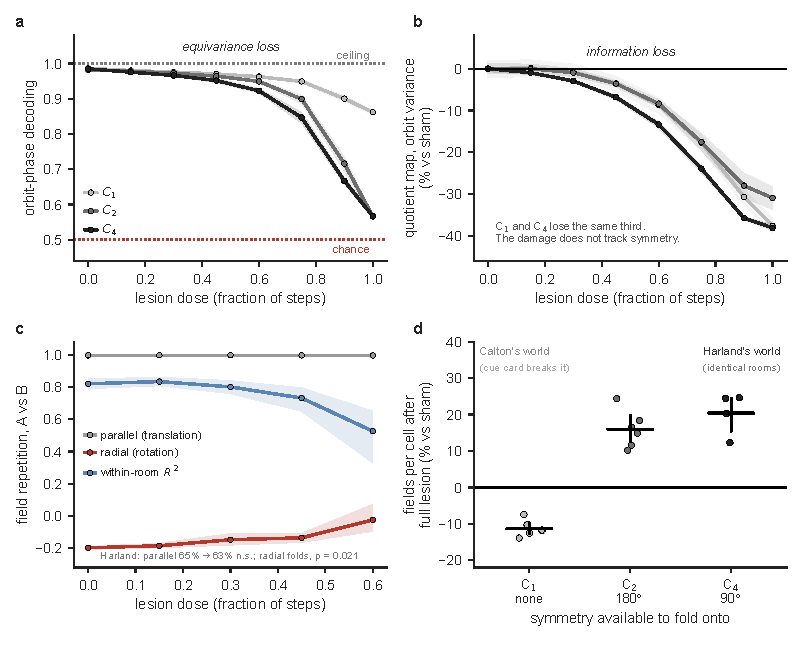
\includegraphics[width=0.86\textwidth]{figures/fig_lesion.pdf}
\caption{\textbf{An in-silico head-direction lesion separates what the compass \emph{tells} the map
from what it \emph{does} to it.} Networks trained with an intact compass, which is then silenced at
test time on a fraction of steps (zeroed, not randomised: an ablated head-direction system carries no
signal, it does not carry a false one). $n = 6$ networks for $C_1$ and $C_2$, $n = 4$ for $C_4$;
shading, $95\%$ bootstrap CI over
networks. (\textbf{a}) \emph{Equivariance loss.} Orbit-phase decoding (which of two
symmetry-related places is the animal in?) collapses to chance in $C_2$ and $C_4$ and holds at
$0.862$ in $C_1$, where no such pair exists ($t = 70.2$, $p = 3\times10^{-19}$). (\textbf{b})
\emph{Information loss.} Orbit variance (is the quotient map still there at all?) falls by about
a third in every arena. The drops are not statistically identical ($F = 10.78$, $p = 0.002$) but they
are not ordered by symmetry: $C_1$ ($-37.6\%$) and $C_4$ ($-38.1\%$) sit at opposite ends of the
symmetry range and lose indistinguishable amounts, while $C_2$ ($-30.9\%$) loses least. Panels (a) and
(b) together are the argument: the same lesion degrades the quotient map without regard to symmetry
and folds it only where a symmetry exists. (\textbf{c}) Harland's $2\times2$, in silico. The
\emph{parallel} arm is the reachable null: a compass is translation-invariant by construction, so it
was never holding those rooms apart, and it does not move ($0.996 \to 0.996$). The \emph{radial}
arm rises. Within-room $R^2$ (blue) is the positive control: it must stay positive, or the repetition
number is two destroyed maps correlating with each other. It does, up to dose $0.6$, and we make no
claim beyond that. (\textbf{d}) Field count after a full lesion, one dot per network: fields
\emph{fall} by $11\%$ where nothing can fold and \emph{rise} by $16\%$ and $20\%$ where something can,
the same dissociation Harland and \citet{calton2003} report in two different worlds.}
\label{fig:lesion}
\end{figure}

\subsection*{One principle, two lesion studies that seem to disagree}

The account also resolves a discrepancy the lesion literature leaves standing. Harland's lesioned place
cells carried less spatial information ($1.29$ to $1.05$ bits per spike) and were less sparse ($0.32$ to
$0.37$), and their fields repeated. Yet anterodorsal and postsubicular lesions leave place-field number
($1.29$ to $1.53$), size, rate and sparsity statistically unchanged, and produce no repetition at all
\citep{calton2003}. Read as claims about what a head-direction lesion does, these disagree. They stop
disagreeing once one asks what world each lesion was performed in. Calton et al.\ recorded in a cylinder
whose inside was ``featureless, except for a white card occupying $\sim 100^\circ$ of arc'', a
polarising landmark at a definite bearing, which breaks the rotational symmetry. Harland's compartments
were identical, behind a black curtain, with no polarising cue: the symmetry stands. A compass lesion
cannot create a symmetry; it can only stop breaking one already there. Where some other channel has
already broken the symmetry, destroying the compass degrades the map and folds nothing; where the compass
was the only thing breaking it, destroying it folds the map. The two studies are the same lesion in two
different worlds, and one principle predicts the null and the positive. The account also predicts an
experience-dependent \emph{unfolding}: \citet{carpenter2015} found that the grid code across two
connected compartments begins repeated and becomes a single global representation with experience. In our
terms the repeated code is the quotient, which unfolds once the animal acquires any cue (a faint
distal landmark, a learned context) that breaks the symmetry the compass could not. The fold is a
starting point set by self-motion, not a fixed endpoint.

\subsection*{The invariant compass is real, and it is not the one the map reads}

The central manipulation of this paper is a compass that carries a full bit of heading yet is
\emph{invariant} under the symmetry (\textit{axis}), set against one carrying the same bit and breaking
it (\textit{parity}). This invites the objection that no such thing exists, that a $G$-invariant compass
is a device built to make a theorem land. It exists. \citet{zhang2022} recorded retrosplenial cells whose own
tuning mirrored the layout's symmetry: bidirectional (two peaks $180^\circ$ apart) in a twofold two-box
($48/575$ cells) and tetradirectional (four peaks at $90^\circ$) in a fourfold four-box ($67/743$).
Three qualifications decide the weight this bears, and we state all three. The comparison across the two
symmetric layouts is between cells, not within them. The comparison that \emph{is} within cell is
against a onefold arena, and there the pattern nearly disappears: of the cells multidirectional in a
symmetric box, only $1/8$ stayed bidirectional and $3/65$ tetradirectional above shuffle. And the
symmetry the cells track is the visual-geometric one: the authors broke the global symmetry with odour
(lemon in one compartment pair, vanilla in the other) and the cells stayed fourfold regardless. The
pattern is learned rather than immediately sensory: absent in naive animals, appearing only after
experience of the layout, and largely surviving darkness ($21/28$ cells in the first dark trial). A
directional signal \emph{approximately} invariant under a symmetry of the environment exists in
mammalian cortex; we say approximately and mean it, and every claim built on it inherits that.
\citet{lachance2024} produce the same object more cleanly, by changing the symmetry and holding the
cells fixed: duplicating a cue card so two identical cards face each other across a square makes
postrhinal head-direction cells fire in two opposite directions ($n = 34$, $W = 1$,
$p = 2\times10^{-10}$) and retrosplenial ones likewise ($n = 37$, $W = 111$, $p = 1\times10^{-4}$),
while entorhinal head-direction cells show no detectable increase ($n = 30$, $W = 207$, $p = 0.62$, a
failure to reject, on a test with no reported power, which we treat as such). The second peak is
reliably weaker than the original ($p = 4\times10^{-5}$ postrhinal, $p = 7\times10^{-11}$
retrosplenial), so the cortical compass is approximately, not exactly, invariant.

This same literature supplies the strongest objection to the account: the invariant compass does not
replace the ordinary one, it \emph{coexists} with it. Classic unidirectional head-direction cells are
recorded in the same retrosplenial tissue, electrophysiologically distinct (peak-to-trough $163\,\mu$s
against $402\,\mu$s), and they never fold. \citet{zhang2022} draw the consequence themselves: ``the
preservation of a global HD signal also allows for the possibility of disambiguation.'' If an unfolded
compass survives, $X$ is available downstream, and the fold should never happen. The objection is
answered by taking the theory literally. The claim is not that \emph{the} compass folds, but that a
predictive code represents $X/G$ where $G$ is the subgroup the self-motion signal \emph{it reads} cannot
break. Two directional populations, one invariant and one breaking, are not an embarrassment; they are
the theory's two conditions realised side by side, and they turn the matter into an empirical question:
which does the hippocampal map read? The lesion answers it. Destroying the head-direction system removes
the \emph{breaking} population; if the map had been reading the invariant channel, the lesion would
change nothing, and instead it folds the map \citep{harland2017}. (We flag that nobody has lesioned the
head-direction system and recorded the invariant cells, so their survival through the lesion is an
assumption of this argument, not a measurement.) Anatomy points the same way but must be stated
narrowly. The multidirectional cells are overwhelmingly a \emph{dysgranular} population
\citep[$76\%$;][]{zhang2022}, and the retrosplenial output characterised by anterograde tracing
terminates in the retrohippocampal region (post-, pre- and parasubiculum and entorhinal cortex)
rather than the subiculum that builds the place map \citep{shibata1994, vangroen1992}. What does
\emph{not} follow is that dysgranular cortex fails to reach the hippocampus at all: \citet{li2025} report
that its one projection to CA1 is \emph{GABAergic}, with no reciprocal excitatory route, and
\citet{sugar2011} decline to read a missing tracing entry as a proven absence. The defensible claim is
the narrow one, that there is no substantial direct \emph{excitatory} route from the cells carrying the
invariant code to the cells building the map, and even it is about Zhang's population only; postrhinal
cortex,
where \citeauthor{lachance2024}'s fold is strongest, \emph{does} project monosynaptically to the
subiculum \citep{naber2001}, and there the work is done by the lesion, not the anatomy.

This forces a correction to how \citet{zhang2022} should be read, including by us. Their
multidirectional cells are not the \emph{antecedent} of the law, the invariant compass whose reading
folds the map. They are its \emph{directional shadow}: a directional code whose tuning has taken on the
symmetry of the group its own input channel cannot resolve. The law applies to them, not through them.
The distinction is not pedantry, and our networks enforce it in both directions. A directional tuning
curve is \emph{not sufficient} to infer a map fold: give a network the \textit{axis} compass in the
$C_1$ arena, with no symmetry at all, and its units are already $93\%$ bidirectional while the map does
not fold (phase $0.971$); put the same compass in the $C_2$ arena and the tuning barely moves ($0.997$)
while the map collapses ($0.552$): the same tuning curve on opposite maps. Nor is it \emph{necessary},
the half we nearly missed: the most completely folded networks, \textit{const} in $C_4$, sit on the
$1/4$ ceiling with \emph{flat} tuning ($m_1 = 0.011$, $m_2 = 0.009$), because a $C_4$-symmetric function
of four headings is a constant. A maximally folded map can present with no directional tuning, and a
completely unfolded one as strongly bidirectional. The consequence is a warning that cuts against every
account, ours included: \emph{no multidirectional tuning curve in cortex licenses an inference about the
hippocampal map}, and neither does its absence. It is also what dissolves the apparent paradox in
\citet{lachance2024}, where the postrhinal compass folds hard while entorhinal grid maps a synapse away
do not move. There is no paradox, because a folded compass upstream says nothing about a map that
reads a different one. It is why the lesion, a fact about the map, is the load-bearing evidence here.
We must be equally clear about a mechanism we do \emph{not} reproduce and cannot rule out:
\citet{alexander2020} propose that an egocentric boundary-vector cell, sampled by an animal that hugs
walls, looks fourfold tuned in a square from directional occupancy alone, with no invariant compass.
Our networks have boundary cells but not the sampling bias. Our agent samples headings near uniformly,
and removing the occupancy correction moves tuning barely at all (\textit{const}/$C_1$ $0.230$ raw
against $0.203$ corrected; \textit{axis}/$C_1$ $0.895$ against $0.929$), so their account is untested
here rather than refuted; settling it needs a thigmotactic agent we have not built. What we
can say is that their mechanism, whatever it explains about \emph{tuning}, has no account of Harland's
lesion, which is a fact about the \emph{map}.

\subsection*{Relation to other models of the spatial code}

The parallel-versus-radial dissociation discriminates among models, because the two arrangements are
built from the same compartments and are locally identical. Any model that fixes firing from local
sensory or boundary geometry must predict the same repetition in both. The sharpest such objection is
that we have rediscovered the boundary-vector-cell account of repetition \citep{grieves2018bvc} with
extra steps; a predictive network does grow boundary-vector cells \citep{uria2020}, and ours are
abundant ($41.6\%$ of units in $C_1$ under \textit{full} are better fit by a boundary-vector cell than
any place field, rising to $61.2\%$ in $C_4$). But a boundary-vector cell is tuned to a wall at an
\emph{allocentric} bearing, and an allocentric bearing is undefined without a compass; as
\citet{julian2018} put it, such models ``assume the existence of a reliable head-direction signal.'' Our
networks show exactly that dependence: ablating the compass drops the boundary-cell fraction from
$41.6\%$ to $14.0\%$ in $C_1$ and $61.2\%$ to $0.8\%$ in $C_4$ (\texttt{bvc\_tuning.csv}), so the
boundary code is built on the compass, not underneath it. The decisive observation is the matched
contrast (Fig.~\ref{fig:bvc}): \textit{axis} and \textit{parity} support comparable boundary populations
($29.2\%$ and $22.1\%$ in $C_2$, \textit{parity} if anything the better fit, $r = 0.482$ against
$0.449$), yet \textit{axis} folds and \textit{parity} does not. Same boundary code, opposite maps,
which no boundary-vector model can produce, because it has no representation of \emph{which} bit the
compass carries. The recent local-feature version of the objection \citep{lachance2024}, that a square
has four walls so a wall detector fires four times, with no compass or symmetry group needed, is
answered on the same ground and two of theirs. The symmetric cortical code does not reach the structures
that would inherit it (the entorhinal head-direction null, $W = 207$, $p = 0.62$, is load-bearing; the
grid null is weaker because a hexagonal lattice is inversion-symmetric). The local-feature and quotient
accounts make identical predictions in a square, and the discriminating shape, one where local features
and global symmetry disagree, the authors themselves name as necessary future work but did not run. And
our own \textit{axis}/\textit{parity} dissociation sees the same walls and folds oppositely.

\begin{figure}[t]
\centering

\includegraphics[width=0.86\textwidth]{figures/fig_bvc.pdf}
\caption{\textbf{Boundary-vector cells are downstream of the compass.} (\textbf{a}) Fraction of
units better fitted by a single idealised boundary-vector tuning curve (a Gaussian over the
distance to the wall at a given allocentric bearing) than by any single Gaussian place field; the
two families have the same free parameters. One dot per network. The network grows boundary cells,
and they require the compass: the fraction falls from $41.6\%$ to $14.0\%$ in the $C_1$ arena and
from $61.2\%$ to $0.8\%$ in the $C_4$ arena as the compass is ablated. (\textbf{b}) The decisive
contrast. Boundary-cell fraction against orbit-phase accuracy, with the group-theoretic floor and
the non-invariant ceiling both drawn. \textit{axis} and \textit{parity} carry the same one bit and
support comparable boundary populations, yet only \textit{axis} folds. Same boundary code, opposite
maps: a boundary-vector model has no representation of \emph{which} bit the compass carries, and so
cannot produce this dissociation.}
\label{fig:bvc}
\end{figure}

Boundary-vector cells are therefore the mechanism a predictive objective discovers; the quotient law
says what any such mechanism can and cannot tell apart. Read the other way, the result
\emph{instantiates} the successor representation rather than competing with it. The successor
representation \citep{stachenfeld2017, momennejad2017successor} is predictive, but over a state space
that is supplied rather than inferred from aliased observations, so whether two symmetric compartments
are one state or two is an assumption, not a result. Under $G$-equivariance, with a $G$-invariant prior
and a policy measurable with respect to the aliased belief, the agent's belief process descends to a
Markov process on $X/G$, because $G$-related states are belief-indistinguishable. This is the
symmetry-induced Markov decision process homomorphism of reinforcement learning \citep{givan2003,
ravindran2004, vanderpol2020}, and the equivalence it induces, in which states are collapsed exactly
because they agree on the entire future, is a bisimulation \citep{ferns2004}, the coarsest abstraction
preserving an MDP's dynamics \citep{li2006}, computed here not by an explicit bisimulation metric but as
the by-product of a network trained only to predict. That the few-percent residual above the floor is a
convergence gap and not a leaky fold is something the input bound settles: Table~\ref{tab:bound}'s
distinguishable fraction is exactly $0.000$ for \textit{axis} and \textit{const} in $C_2$, so the
observations are \emph{exactly} bisimilar and the residual can only be the network's finite-training
approximation of the exact quotient, sitting near the quotient ceiling rather than the un-quotiented one
(Table~\ref{tab:phase}). Two learned-map models place against the same test. The clone-structured
cognitive graph \citep{george2021, raju2024} disambiguates aliased observations by transition context
and reproduces repetition, but not the dissociation: run without a compass, \citet{raju2024} report that
``place field repetition persists in the modified layout,'' folding even when the rooms are rotated.
They then supply the fix themselves, that ``an external head direction input'' makes the different
orientation give unique place fields. That is our claim, reached independently in a model with no
boundaries and no metric. The Tolman--Eichenbaum machine \citep{whittington2020tolman} factorises a
structural code that is a function of the action sequence, and an action code invariant under the
arena's symmetry folds it as ours folds, so the two agree on the effect and differ only in mechanism.
The symmetry itself has been noticed before: \citet{jeffery2023} observes that repetition between
same-orientation compartments ``is a translational symmetry, which echoes the translational symmetry of
the environment,'' while ``the head direction signal has a rotational asymmetry.'' That is the intuition
this paper formalises. What is new is not the observation but the derivation: that the relevant object
is the subgroup of the environment's symmetry the self-motion signal fails to break, that a learned
predictive code must collapse onto its quotient, that the collapse is bounded at $1/|G|$, and that what
governs it is equivariance rather than information, so two encodings carrying the same single bit come
apart completely (Table~\ref{tab:models}).

\begin{table}[t]
\centering
\small
\setlength{\tabcolsep}{4pt}
\caption{Where models of the spatial code stand on the symmetry dissociation. The decisive column
is the last: the parallel and radial arrangements are locally identical, so any model that reads
firing from local geometry or the current observation predicts the same repetition in both, and
cannot produce the dissociation that \citet{grieves2016} observed.}
\label{tab:models}
\begin{tabular}{p{0.30\textwidth}p{0.15\textwidth}p{0.18\textwidth}p{0.25\textwidth}}
\toprule
model class & fields learned from experience & repetition in identical rooms &
parallel-vs-radial dissociation \\
\midrule
Continuous attractor / path integration \citep{burak2009, sorscher2023unified}
& metric built in & not addressed & no \\[3pt]
Boundary-vector / geometry \citep{hartley2000}
& partly & yes & no (predicts repetition in both) \\[3pt]
Successor representation \citep{stachenfeld2017}
& yes (predictive) & depends on the given state space & not addressed \\[3pt]
Clone-structured graph \citep{george2021,raju2024}
& yes (transition clones) & yes (aliased views share clones) & no: repeats in \emph{both}
without a compass \citep{raju2024} \\[3pt]
Tolman--Eichenbaum machine \citep{whittington2020tolman}
& yes (structural) & yes, if the action code is symmetry-invariant & consistent \\[3pt]
Reconstruction / autoencoder (this work, control)
& yes & yes & no (predicted; folds every encoding alike in the rotational arena, $p=0.59$;
not run on the compartment mazes) \\[3pt]
Predictive RNN \citep{levenstein2024}, this work
& yes (emergent) & yes & \textbf{yes}, set by HD invariance \\
\bottomrule
\end{tabular}
\end{table}

\subsection*{What the model reproduces, and what it does not}

Table~\ref{tab:bio} scores the model against the animal literature. Most rows are reproduced without
fitting, but three kinds of departure are worth naming. The two rows marked \emph{absent} are
architectural: head direction enters as an oracle input rather than being learned, and no non-negativity
constraint is imposed, which is the condition under which hexagonal grids emerge in trained path
integrators \citep{sorscher2023unified}. Nothing here bears on the ring or toroidal manifolds of
entorhinal cortex, and we make no claim about them.

\begin{table}[t]
\centering
\small
\setlength{\tabcolsep}{4pt}
\caption{The model against the animal literature. ``Reproduced'' means the model shows the
phenomenon without being fitted to it; ``absent'' means the phenomenon cannot exist in this
architecture and we do not claim it; ``tested, not found'' means the architecture could in
principle show the phenomenon but a direct test did not find it.}
\label{tab:bio}
\begin{tabular}{p{0.29\textwidth}p{0.22\textwidth}p{0.28\textwidth}p{0.11\textwidth}}
\toprule
observation in animals & source & in this model & verdict \\
\midrule
Fields repeat across translationally related identical compartments; path integration does not
separate them
& \citet{spiers2015} & translation leaves the compass invariant, so the code folds onto $X/G$
& reproduced \\[4pt]
Repetition in parallel compartments, markedly less in radial ones; survives removal of the
orientation landmark; attributed to self-motion
& \citet{grieves2016} & rotation makes the compass equivariant, so the code lifts
& reproduced \\[4pt]
Place fields repeat across the arms of a hairpin maze, and the repetition is
running-direction dependent
& \citet{derdikman2009} & folding onto $X/G$ makes one unit fire at all $|G|$ orbit-mates, and
the direction dependence is the compass entering the fold, but we have not built and run a
hairpin-maze arena to test this directly
& consistent \\[4pt]
Anterodorsal and postsubicular lesions leave place-field number, size, rate and sparsity
unchanged, and lower coherence, in a cylinder polarised by a cue card
& \citet{calton2003} & his cue card breaks the rotational symmetry, so his is our $C_1$ arena and
there is nothing for the lesion to fold onto: silencing the compass there leaves the mean rate
unchanged, lowers coherence, and crucially does \emph{not} multiply fields, in flat contrast to the
symmetric arenas. But it does not leave field count untouched either: ours \emph{falls} by
$11.3\%$ ($p = 0.031$, $n = 6$), where his is unchanged with a point estimate that rises
($1.29 \to 1.53$, n.s.)
& partly: the \emph{absence of multiplication} is reproduced, the field count itself is not,
and the sign is wrong \\[4pt]
The same lesion \emph{raises} in-field directional information ($0.25 \to 0.48$ bits per spike)
& \citet{calton2003} & \textbf{not reproduced.} Ours falls to near zero. In our network the compass
is an additive input coordinate, so a unit's directional tuning is inherited from it and must vanish
with it. Calton et al.\ propose the opposite role, that head direction \emph{cancels} the
directionality of egocentric views and binds them into an allocentric code, so that removing it
causes ``directional fragmentation''. Ours is a model of what the compass makes representable, not
of how it binds views, and this readout is outside what it can speak to
& mismatch \\[4pt]
Two visually identical boxes, walked between, are not distinguished when related by a translation
and remap completely when related by a $180^\circ$ rotation
& \citet{fuhs2005} & the compass is invariant under the first group element and equivariant under
the second; the compartment networks repeat under translation and lift under rotation
& reproduced \\[4pt]
Head direction plus recurrence plus prediction are needed for offline replay
& \citet{levenstein2024} & offline trajectories exceed the coverage of a wake path of equal
length only with the full compass and $k \ge 1$; coverage falls monotonically as the compass
is ablated ($1.30 \to 0.80 \to 0.45 \to 0.31 \times$ wake), and the autoencoder never leaves
$0.37\times$. Replay appears at the same horizon as symmetry resolution and improves no
further with a longer one
& reproduced \\[4pt]
A predictive objective is sometimes read as implying prospective (anticipatory) place coding
& --- & rebuilding each rate map on the position up to five steps ahead does not sharpen it at
any prediction horizon; the network's predictive character shows up in offline replay, not in a
spatial lead of its fields
& tested, not found \\[4pt]
Rate remapping: a slight rate-based discrimination between otherwise repeated fields
& \citet{spiers2015} & the pure predictive model folds almost completely (repetition $+0.997$,
compartment decodable only at $0.515$ against a chance of $0.5$); a graded-cue sweep (Discussion) found no
rate-based discrimination at any cue strength and no departure of repetition from ceiling; a
small, chance-exceeding room-decode residual is present already at zero added cue
& tested, not found \\[4pt]
Grid cells on a toroidal population manifold, invariant across environments and sleep
& \citet{gardner2022toroidal} & no grid cells (full compass, gridness $\le 0.08$); the torus cannot exist here
& absent \\[4pt]
Head-direction cells lie on a ring manifold that matures before place and grid coding
& \citet{taube1990, langston2010} & head direction is supplied as a four-point input, not learned
& absent \\
\bottomrule
\end{tabular}
\end{table}

The row marked \emph{tested, not found} is the one place the model and the animals part on the fold
itself. Spiers reported repetition \emph{with} a slight rate-based discrimination; our network, given
perfectly identical rooms, keeps none, and folds to within a small residual. Because real compartments
are never perfectly identical, we reasoned a cognitive map should collapse toward $X/G$, not exactly
onto it, and tested whether a symmetry-breaking channel too weak to lift position would still modulate
rate, the signature Spiers reported. Eq.~\ref{eq:bound} lets that curve be predicted before training. A first
attempt (a uniform brightness shift) gave a step rather than a ramp, so we replaced it with fixed
per-pixel Gaussian noise competing against a room-B tint swept to target single-step discriminabilities
evenly over $d' \in \{0,\dots,3\}$ (Methods). Both a generalisation and a within-trajectory room decoder
then rise smoothly with $d'$ (Spearman $\rho = 0.92$ and $0.99$, $n = 64$, $p < 10^{-25}$; $d'=0$ vs
$d'=3$, $p = 0.000155$), so the sweep tests the prediction as designed. The prediction is not borne out.
Field-shape repetition stays at ceiling across the sweep ($\approx 0.997$, $p = 0.88$, $\rho = 0.17$),
and a rate-asymmetry readout is flat throughout ($p = 0.88$, $\rho = 0.02$): no evidence of a rate-based
signal, let alone one that leads position. This is an honest negative on the rate-leads-position
prediction, as pre-registered. Reconciliation with Spiers' partial fold has to come, in this
architecture, from the residual already present at zero added cue (generalisation room decode $0.510$,
above chance, Wilcoxon $p = 0.023$, $n = 8$), not from a graded rate-versus-position dissociation: some
trace of compartment identity survives even the perfectly-identical limit, but it does not grow into a
rate code as the cue strengthens.

\subsection*{Limitations}

A first group of limitations are architectural absences on the same footing as the missing grid torus.
The arenas are discrete $18\times18$ grids with four headings, so the head-direction ``ring'' has four
points and no continuous topology; nothing here speaks to the toroidal manifolds of entorhinal cortex
\citep{gardner2022toroidal}, and the place-like but not grid-like tuning (full-compass gridness: mean
$-0.29$, maximum $+0.08$, none above $0.3$; invariant encodings can reach $0.50$ through
symmetry-induced field repetition rather than hexagonal tuning) is expected given a supplied compass and
no non-negativity constraint \citep{sorscher2023unified}. The network has no membrane dynamics, spikes,
theta, or excitatory--inhibitory separation, and is trained once on a fixed arena, so it speaks to the
representation a predictive objective converges to, not to drift across sessions; all results use one
architecture (hidden size $500$, horizon $k=5$), and hidden and arena size are not swept.

A second group are empirical departures from biology, most already bounded by a control. The supplied
compass is tested by the $30\%$-corruption and learned-compass results; what is not modelled is a
continuous compass that drifts and is re-anchored over time. Real open-field place cells are largely
omnidirectional \citep{mcnaughton1983, markus1995}; this model's units are only partly so
(opposite-heading rate-map correlation, \textit{full}, $C_1$: mean $0.56$, median $0.64$, $35\%$ of
pairs above $0.8$), because head direction enters as a direct input rather than being merged away
upstream. A proposed topology-before-geometry developmental order does not hold here under a shuffle null
(position is linearly decodable at $R^2 = 0.79$ before training), so we make no such claim, and place
fields do not anticipate future position (Table~\ref{tab:bio}).

A third group bound how far the results generalise. Symmetry here is a property of the landmark layout,
not the arena geometry, which is square in every condition, so only the $C_1$/$C_2$/$C_4$ arenas satisfy
the Theorem's hypotheses exactly; the compartment mazes are an empirical demonstration of the same
principle rather than a strict instance, since the connecting corridor lacks the group's cyclic closure
(a temporal-conditioning analysis rules out corridor memory as the alternative, Methods). A sharper
control asks whether room decodability on the compartment maze rises with horizon: for $k \in \{0,1,3\}$
($n = 8$ each) steady-state room decodability stays at chance ($0.508$, $0.502$, $0.510$; Spearman
$\rho = 0.07$, $p = 0.73$) while repetition holds near ceiling ($0.98$--$0.99$), supporting
architecture-robustness over horizon-limitation, though $k = 5$ and $k = 10$ remain untested. And the one
real-neuron test here, the CA1 city-block reanalysis, is exploratory rather than diagnostic: a
conjunctive place-by-direction code predicts the same correlation, two controls confirm the accounts are
not separable in these data, and we treat the model's own prediction, not the reanalysis, as the
evidence.

\subsection*{Outlook}

The appeal of predictive learning is that a single domain-general objective, predict the next
observation, grows structured spatial representations with no hand-built spatial prior, in artificial
networks as in the hippocampus \citep{levenstein2024, stachenfeld2017}. What this study adds is that the
geometry of the learned code is then set by the symmetry structure of the agent's interaction with the
world, the group action of the environment on the self-motion signal, rather than by the architecture.
That makes the paradigm a controlled developmental probe: because the representation is learned, each
factor that shapes it in an animal, and is there confounded or fixed, becomes a variable that can be
turned on its own, whether the geometry of the enclosure, the information and invariance of the
self-motion signal, the locomotor policy, or the training task.

Two experiments follow immediately, both within reach of a laboratory already equipped for them. The
first is a prediction we would stake the account on, and it is sharper than it looks because the law
makes \emph{two different} predictions in one apparatus. \citet{lachance2024} showed that two identical
cue cards on opposite walls make postrhinal and retrosplenial head-direction cells bidirectional, a
cortical compass invariant under a $180^\circ$ rotation. The tempting move is to predict a fold and go
record place cells there. That would be wrong, and the account says why: in the same animals, entorhinal
head-direction cells did \emph{not} become bidirectional ($W = 207$, $p = 0.62$), so the classical
compass, carried forward by path integration, still breaks the symmetry, and the classical compass is
the one the map reads. In an \emph{intact} rat the two-cue square should therefore produce no fold, but
\emph{anchoring}: with the animal disoriented, the map must choose between the two $180^\circ$-related
gauges the scene allows, and should adopt one at chance, which is what \citet{keinath2017} report. The
fold appears only when the breaking compass is removed. The experiment is the crossing of two apparatuses
that already exist: $\{$one cue, two cues$\} \times \{$sham, head-direction lesion$\}$. Repetition is
predicted in exactly one of the four cells (two cues, lesioned), with nothing free to fit. Two are
already observed: the intact single-cue square is an ordinary place map, and the lesioned single-cue
square is \citet{calton2003}, who found no multiplication of fields because a cue-controlled arena has no
symmetry to fold onto. Two assumptions do work here and we would rather name them: that the hippocampus
is dominated by the classical breaking compass rather than the folded postrhinal one (the lesion shows
the map reads \emph{a} breaking compass, not \emph{which}, and postrhinal cortex reaches the subiculum
monosynaptically \citep{naber2001}), and that the entorhinal null holds in a session entered from a
single-cue baseline, whereas the anchoring prediction requires between-session disorientation, so the
design must specify which it is. The cortical fold also shows hysteresis \citep{lachance2024}, so the law
is a claim about a \emph{learned} map, and the conditions must be counterbalanced rather than run in
sequence. The fourth cell, two cues and lesioned, is the one genuinely open, and it is the one the
account stands on; a null there would be a serious problem for us, and we say so. Neither
\citet{lachance2024} nor \citet{zhang2022} recorded a place cell, and the laboratories holding the lesion
and the place cells \citep{harland2017} are not the ones holding the cue-duplication apparatus. The
experiment is a collaboration away, not a decade.

The second is a control the model can run and the field has not. In \citet{zhang2022} the local shape of
each compartment is confounded with the global symmetry of the layout: the fourfold environment is built
of \emph{square} compartments and the twofold one of \emph{rectangles}, so a code tracking local walls
and a code tracking global symmetry predict the same thing. The confound is severable in simulation, and
only there without years of rat training: build a fourfold layout out of compartments whose own shape has
no fourfold symmetry, and ask whether the compass and the map follow the global group or the local
geometry. The same severance answers \citet{lachance2024}, whose authors name such a shape as necessary
future work but did not run one. We have not run it here, and it is the first thing we will run next.
Progressively more biological designs (a learned compass allowed to drift, non-negative rates, separate
path-integration and sensory streams, planning modules) would then let one ask which ingredients are
necessary for the joint emergence of place and grid cells, turning the catalogue of spatial cell types
into consequences that follow from an objective, an architecture, and an experience, of which the
symmetry-driven fold reported here is one.

\section{Methods}

\paragraph{Architecture and training.} We use \texttt{pRNN\_th} \citep{levenstein2024} unchanged:
a layer-normalised recurrent cell, hidden size 500, truncation $T = 200$, rollout horizon $k=5$
unless stated, observation size 147 ($7\times7\times3$), action size 5. Training uses RMSprop
($\alpha = 0.95$, $\epsilon = 10^{-6}$) with four parameter groups at per-group learning rates
$\lambda\sqrt{1/H}$ for $W_{\text{rec}}, W_{\text{out}}$, $\lambda\sqrt{1/(n_{\text{obs}} +
n_{\text{act}})}$ for $W_{\text{in}}$ and $0.1\lambda$ for the bias, with bias-only weight decay;
$\lambda = 2\times10^{-3}$, batch size 8, gradient clipped per model to norm 1, 80{,}000 steps.

\paragraph{Arenas.} $18\times18$ MiniGrid arenas (324 positions) with landmark layouts of $C_1$,
$C_2$ and $C_4$ rotational symmetry. The observational discriminability index (ODI; the Spearman
correlation between heading-averaged observation distance and spatial distance across all pairs
of positions) is \emph{not} matched across the three arenas, and cannot be: symmetric landmarks
make distinct positions observationally identical, so discriminability necessarily falls with
symmetry order. Measured over all 324 positions, $\mathrm{ODI} = 0.336$ ($C_1$), $0.288$ ($C_2$),
$0.262$ ($C_4$).

This does not confound the results, for two reasons. The decisive contrast, \textit{axis} vs.\
\textit{parity}, is made \emph{within} one arena, on the same trajectories, so the observation
stream and its ODI are identical between the two arms; the only difference is a $4\times4$ matrix
on the heading block. And across arenas, ODI does not predict the readout: with a full compass,
phase decoding is $0.981$, $0.978$ and $0.984$ for $C_1$, $C_2$, $C_4$ (Pearson $r=-0.37$ against
ODI, $p=0.76$, $n=3$ arenas), with the least discriminable arena scoring highest. Trajectories:
10{,}000 per arena, 200 steps, random start position and heading. The policy is a fixed-probability
random walk (forward $0.60$, turn left $0.15$, turn right $0.15$, stop $0.10$), identical at every
position, heading, and arena; nothing about it depends on which copy of the fundamental domain the
agent occupies, which is what makes it measurable with respect to the agent's belief (Theorem).

\paragraph{Head-direction encodings.} The heading block of the action vector is left-multiplied
by a fixed $4\times4$ matrix: identity (\textit{full}); $\tfrac12(I + P^2)$ where $P$ is the
cyclic shift (\textit{axis}); the block-averaging matrix pairing $\{E,S\}$ and $\{W,N\}$
(\textit{parity}); and $\tfrac14\mathbf{1}\mathbf{1}^\top$ (\textit{const}). Column sums are
preserved, so activation magnitude is unchanged. Entropies under a uniform heading prior are
$2, 1, 1, 0$ bits.

\paragraph{Ensemble training.} All networks sharing a computation graph (arena, encoding and seed
all leave it unchanged; the horizon $k$ does not) are trained as a single job using
\texttt{torch.func.stack\_module\_state} with \texttt{vmap(functional\_call)}, which lowers every
per-model matrix multiply to one batched multiply and makes the kernel-launch count independent
of the number of models. Forward passes are bit-exact against separate runs; gradients are
bit-exact with noise disabled and agree to $2.3\times10^{-10}$ absolute with the production noise
on (\texttt{bmm} reassociation). Per-model gradient clipping, the four-group RMSprop and the
sum-of-per-model-means loss are all preserved; each is checked against the reference
implementation by test.

Ensemble sizes differ across analyses, and each figure and table states its own $n$: the orbit-phase
and quotient-geometry results use the full sweep ($n=10$ per encoding in $C_1$ and $C_2$, $n=8$ in
$C_4$; $112$ networks in all), whereas the $C_4$ four-way ceiling (Table~\ref{tab:c4}) and the
per-network fold and lesion analyses (Fig.~\ref{fig:fold}, Fig.~\ref{fig:lesion}; $n=6$ in $C_1$ and
$C_2$, $n=4$ in $C_4$) use smaller matched subsets.

\paragraph{Orbit-phase decoding.} Hidden states are collected over 20{,}000 raw timesteps (no
per-position averaging); repeated visits to one position therefore contribute multiple, slightly
different rows, and \texttt{GroupKFold} groups every row from an orbit's two positions together
regardless of how many visits each contributed. Orbits are $\{x, R^2x\}$ under the $180^\circ$
rotation (or the four-element $C_4$ orbits where stated); the arena side is even, so no rotation
has an integer fixed point and every orbit has exactly $|G|$ cells (162 orbits at $C_2$, 81 at
$C_4$). Phase labels are balanced, and cross-validation folds hold out whole orbits, so the decoder
must generalise a phase direction rather than memorise orbits or exploit a repeated visit to the
same position appearing on both sides of a split. We report the accuracy of a logistic decoder,
together with the $R^2$ of ridge decoders for the raw position and for the position within the
fundamental domain. The latter is not a positive control (recovering a folded coordinate from an
unfolded code requires a nonlinear map), so the sanity check that a code still represents space is
$\max(R^2_{\text{raw}}, R^2_{\text{domain}})$.

We checked directly whether this pipeline is itself biased, since a 500-dimensional feature decoded
by 5-fold \texttt{GroupKFold} over only 162 orbit groups is a regime where an improperly validated
decoder could read above chance on a truly invariant code. The standardiser is fit on the training
fold only (never on the pooled data before the split), and no other preprocessing step (no PCA, no
whitening, no cross-validated regularisation strength) touches held-out rows before scoring, so
there is no pre-split leakage in the code. We also ran the decoder on a synthetic code matched to
this exact regime, 500 dimensions, 162 $C_2$ orbits, 20{,}000 rows, constructed to be exactly
invariant to phase by hand: it reads $0.498$, indistinguishable from the nominal $0.500$. The
decoder is therefore unbiased in the regime this paper uses it in. The $k{=}0$ full-compass
condition's $0.536$ and every folded network's $0.52$--$0.56$ (Table~\ref{tab:phase}) are not,
consequently, a decoder artefact to be read against as an empirical floor; they are real signal in
the trained networks themselves, a small residual above the nominal chance the permutation test
above confirms is not noise. We attribute it, as in the Discussion, to finite training never
reaching the exactly invariant solution a population-level, infinitely-trained network would.

\paragraph{Within-episode phase (Experiment 0).} The across-episode analysis above shows absolute
orbit phase is undecodable in steady state, but that alone cannot distinguish a code that never
carries phase information from one that carries it locally, right after an episode begins, and
loses it as the trajectory accumulates. We tested this directly with a per-episode-relative label,
$z(t) = \text{phase}(t) \oplus \text{phase}(0)$, decoded with a logistic model under
\texttt{GroupKFold}-by-episode and \texttt{class\_weight='balanced'}, reporting balanced accuracy
(chance $=0.5$ regardless of $z$'s base rate) as a function of dwell time since episode start. An
earlier version of this analysis, reporting raw accuracy, was invalidated by a majority-class
confound: under a random walk, $P(z=1)$ rises from about $0.08$ near episode start to about $0.46$
by $100+$ steps purely from position continuity, independent of the hidden state, so a
majority-class-only classifier scored about $0.93$ at $0$--$10$ steps using zero real information;
comparing every reported number against this baseline is now standard in the pipeline.
The corrected result, $n=10$ seeds each of \textit{learned}, \textit{axis} and \textit{const} in
the $C_2$ arena, is nominally above chance (Wilcoxon signed-rank against $0.5$, exact two-sided,
uncorrected) at every dwell bin tested for all three encodings, decaying from
$0.66$--$0.74$ near episode start toward the across-episode baseline ($0.52$--$0.53$) by
$100+$ steps. The effect at the longest bin is markedly weaker for \textit{learned}
($p=0.049$, at the edge of detection) than for \textit{axis}/\textit{const} ($p \le 0.0098$),
though none actually falls to non-significance. The fold is therefore decodable-but-drifting: the
network keeps a locally coherent orbit-frame for a window after an episode starts, which
attenuates toward the steady-state floor rather than vanishing at the first step (an instantaneous
fold) or never appearing at all (a code with no phase information to lose).

\paragraph{Isotypic spectrum.} Each unit's rate map is decomposed into the four characters of
$C_4$; $P_k$ is the normalised power in character $k$, $\sum_k P_k = 1$, and $P_1 = P_3$ for real
maps. $\mathrm{RA} = P_0 - P_2$ and $\mathrm{odd} = P_1 + P_3$.

\paragraph{Compartment mazes.} Room-interior observational identity (two and four rooms) is verified
by direct enumeration: rendering every room-interior cell and heading and comparing pixel images
across rooms gives zero mismatch (0/144 pairs, two rooms; 0/432, four rooms). The connecting corridor
is not: because every room's corridor opens onto one shared junction, a room at either end of the
junction's span sees it truncated on one side while an interior room does not, and once the agent's
forward view (F cells) reaches far enough into the corridor to include the junction, this asymmetry
becomes visible (maximum single-channel pixel mismatch of 5/255, first appearing exactly where the
view depth reaches the junction column). Room-interior views therefore satisfy the aliasing
this maze is built to test; the maze as a whole, corridor included, does not instantiate a finite
group acting freely on the full state space the way the rotationally symmetric $C_2$/$C_4$ arenas
do, so the two- and four-room results are an empirical demonstration of the same principle rather
than a direct instance of the Theorem. Room decoding (\texttt{label\_rooms}) is restricted to
room-interior timesteps for exactly this reason.

The two-room arrangements compound this: the corridor connecting the compartments is not the same
length in both. The translation arrangement's doors are joined by a direct link ($27$ cells,
door to door); the rotation arrangement's link runs around three edges of the arena to avoid
cutting through the rotated room's wall ring ($57$ cells; $58$ non-room cells in total against
$28$ for translation). A longer, more distinctive corridor is a channel by which recurrent memory
of the just-completed transit, not the compass, could carry room identity into the following
room-interior states, which would confound the translation/rotation contrast with corridor length
rather than isolating head-direction equivariance. We tested this directly on the trained networks
by conditioning room decoding on the number of steps since the animal last crossed into its current
room. The two arrangements show opposite temporal signatures. Under translation, decoding is
above chance immediately on entry ($0.56$ within the first two steps) and decays to the
near-chance floor within about ten steps ($0.51$, matching the steady-state value reported in the
main text); a corridor-memory trace is real but small and transient. Under rotation, decoding is
\emph{below} its ceiling immediately on entry ($0.71$) and \emph{rises} to it over the following
several steps ($0.92$, $0.98$, $0.99$ at $2$--$5$, $5$--$10$ and $10+$ steps; \texttt{corridor\_dwell.csv}).
A corridor-memory account predicts the opposite ordering, highest immediately after the longer
transit and decaying, so it does not explain the rotation result; the rise instead matches a
network that needs a few steps of position-and-heading integration after entry to resolve which
room it is in, consistent with the compass account this maze is built to test. The corridor-length
asymmetry is therefore a real, small, and transient confound specific to the translation
arrangement, not an alternative explanation for the dissociation itself: it makes the reported
translation number (averaged over all room-interior timesteps, including the contaminated first
few) a slightly conservative estimate of the steady-state fold, and it does not touch the rotation
result at all.

\paragraph{CA1 reanalysis.} From \citet{hockeimer2023} (JHU repository doi:10.7281/T15HMQD4,
\texttt{AlleySuperpopDirVisitFiltered.csv}) we took, for each place field, its per-visit firing
rates split by travel direction, and formed a directional index $\mathrm{DI} = (r_+ - r_-)/(r_+ +
r_-)$ with $+/-$ the two directions of the field's alley (E/W for horizontal alleys, N/S for
vertical); fields with fewer than three visits in either direction were dropped. The primary
statistic is the Pearson correlation over within-cell same-orientation field-DI \emph{pairs}
(a cell's repeating fields lie in translation-related alleys). The shuffle null permutes DI values
across all repeating fields \emph{within an orientation}, breaking the assignment of DIs to cells
while preserving the marginal DI distribution, and is recomputed $2000$ times. This null, however,
also destroys cell-level directionality, so we ran two further controls that hold it fixed. First,
the same correlation on \emph{non-repeating} cells' same-orientation fields (which the fold does
not predict should correlate). Second, a directionality-matched scramble that preserves each cell's
per-orientation mean DI and resamples the within-cell residuals from the global pool, isolating the
between-cell (global-directionality) contribution; the directional index is substantially a
between-cell property (mixed-effects ICC $0.31$), and this scramble reproduces (indeed exceeds) the
observed correlation. The observed correlation is
therefore consistent with the quotient but not separable from a conjunctive place-by-direction code
in these data; we report it as such.

\paragraph{Statistics.} All contrasts are two-sided exact Mann--Whitney $U$ tests on per-network
values. The planned contrasts are \textit{axis} vs.\ \textit{parity} within each arena, at
$n = 10$ per cell for s1 and s2 and $n = 8$ for s4; at $n = 10$ vs.\ $10$ the exact two-sided
floor is $2/\binom{20}{10} = 1.1\times10^{-5}$, and a $p$-value at that floor indicates complete
separation (every network in one group above every network in the other). Bonferroni correction
across the three planned arena contrasts is applied where stated. Secondary experiments carry
their own $n$: the prediction-horizon and noisy-compass sweeps use $n = 6$ per cell (floor
$0.00216$), the isotypic re-run $n = 5$ (floor $0.0079$). Folded decoding accuracies are compared
to their $1/|G|$ floor by a one-sample $t$-test where a residual is claimed. No results were
excluded; models failing a criterion are reported as such rather than dropped.

\section*{Data and code availability}

The source data underlying every figure and table are provided as comma-separated files in
\texttt{project5\_symmetry/Report/data/}; a per-file index maps each reported value to its
source (\texttt{Report/data/README.md}). All code, the analysis pipeline that regenerates those
files from trained checkpoints, and the figure-generation scripts are openly available at
\url{https://github.com/RavulapalliManas/Thesis_work} (\texttt{project5\_symmetry/}), and will
be archived on Software Heritage on acceptance. The test suite pins the claims that fail
silently: the bit-exactness of the batched ensemble against per-model training, that the $k=0$
target is exactly the anchor observation, that a synthetic $C_2$-folded code reads chance phase
while a code with no spatial signal is distinguishable from it, and that the isotypic identity
$\mathrm{RA} = P_0 - P_2$ holds. Trained checkpoints and raw trajectories ($\sim$40\,GB) are
available from the author on request; every published number is reproducible from the committed
data files without them.

\section*{Author contributions}
M.V.S.R. designed the study, implemented the models and analyses, ran the experiments and wrote
the manuscript.

\section*{Competing interests}
The author declares no competing interests.

\section*{Use of AI tools}
Large language models were used for code review, refactoring, and drafting assistance. All
experiments, statistics and scientific claims were specified, executed and verified by the
author; every number reported here is produced by the archived analysis scripts.

\bibliography{../references}

\end{document}
